\documentclass[aspectratio=169]{ctexbeamer}
\definecolor{urls}{RGB}{137, 180, 250}
\definecolor{link_text}{RGB}{245, 224, 220}
\hypersetup{
  colorlinks,
  linkcolor=, % This config controls the jumps inside the pdf
  urlcolor=urls,
}
\renewcommand{\UrlFont}{\ttfamily\scriptsize}

\usetheme{AnnArbor}
\usepackage[style=Mocha,accent=Rosewater]{beamercolorthemecatppuccin}

\usefonttheme{serif}
\usefonttheme{professionalfonts}

\usepackage[T1]{fontenc}
\setmainfont{LXGW WenKai}
% \setmainfont{Cascadia Code NF}
% \setsansfont{}
\setmonofont{Cascadia Code NF}
\usepackage{xeCJK}
\setCJKmainfont{LXGW WenKai}
% \setCJKmainfont{}
\setCJKmonofont{Cascadia Code NF}
\newcommand{\nerd}[1]{\texttt{#1}}
\setmonofont{Cascadia Code NF}[
  Contextuals=Alternate
]

\PassOptionsToPackage{hyphens}{url}
% \usepackage{ulem}
\usepackage{graphicx}
%\usepackage{wrapfig}
\usepackage{pifont} % Symbols used as itemize symbols
\usepackage{enumitem}
\setlist[itemize,1]{label={\small\color[RGB]{242, 205, 205}\ding{111}}}
\setlist[itemize,2]{label={\footnotesize\color[RGB]{242, 205, 205}\ding{111}}}
\usepackage{float}
\usepackage{booktabs}

\setbeamerfont{footnote}{size=\tiny}
\setbeamertemplate{footnote}{%
  \color[RGB]{108, 112, 134}%
  \insertfootnotetext%
}
\setlength{\footnotesep}{0.3\baselineskip}
\newcommand{\refnote}[1]{\footnotetext{#1}}

\usetheme{AnnArbor}

\usepackage{pifont}

\usepackage{amsmath, amssymb, amsthm}
\usepackage{listings}
\lstdefinestyle{bash}{
  alsoletter=-,
  keywordstyle=[2]{\color[RGB]{243, 139, 168}},
  morekeywords=[2]{sudo},
  keywordstyle=[3]{\color[RGB]{166, 227, 161}},
  morekeywords=[3]{add-apt-repository, apt-get, apt},
  keywordstyle=[4]{\color[RGB]{250, 179, 135}},
  morekeywords=[4]{install},
}
\lstdefinestyle{lua}{
  alsoletter=-,
  keywordstyle=[2]{\color[RGB]{137, 180, 250}},
  morekeywords=[2]{name, priority, opts, config, dependencies, submodules, main, version, init, number, boolean},
  keywordstyle=[3]{\color[RGB]{180, 190, 254}},
  morekeywords=[3]{fun, setup},
  keywordstyle=[4]{\color[RGB]{250, 179, 135}},
  morekeywords=[4]{},
}
\lstdefinestyle{path}{
  alsoletter=~,
  basicstyle={\footnotesize\ttfamily\color[RGB]{147, 153, 178}\itshape},
}
\lstset{
  language={[5.1]lua},
  style=lua,
  basicstyle=\footnotesize\ttfamily,
  breaklines=true,
  showstringspaces=false,
  breakatwhitespace=true,
  keywordstyle=\color[RGB]{245, 169, 127},
  numberstyle={\ttfamily\color[RGB]{110, 115, 141}},
  commentstyle={\color[RGB]{147, 153, 178}\itshape},
  stringstyle={\color[RGB]{166, 218, 149}},
}
% NOTE: \lstinline{} command does not support background color
\lstdefinestyle{nvim}{
  alsoletter=:,
  keywordstyle=[3]{\color[RGB]{166, 227, 161}},
  morekeywords=[3]{:Tutor, :help}, % ChkTeX 26
}

\newcommand{\TODO}[1]{\textcolor{red}{TODO\@: #1} }

% \newcommand{\link}[3][]{\href{#3}{#2}\footnote[#1]{\url{#3}}}
\newcommand{\link}[3][]{\href{#3}{#2\textsuperscript{\nerd{}}}}

\title{Neovim从入门到出门}
\subtitle{第七节:界面美化(二)}
\author{Jacky-Lzx}
\date{\today}

\usepackage{tikz}
\titlegraphic {
  \begin{tikzpicture}[overlay,remember picture]
    \node at (-6, 4.5){
      
\includegraphics[height=1cm]{./Figures/Neovim_logo.png}
    };
    \node at (6, 4.5){
      
\includegraphics[height=1cm]{./Figures/Catppuccin_logo.png}
    };
  \end{tikzpicture}
}

\usepackage{makecell}

% ChkTeX-file 19
\begin{document}

\begin{frame}
  \titlepage
\end{frame}
\begin{frame}{大纲}
  \tableofcontents
\end{frame}
% Current section
\AtBeginSection[ ] {
  \begin{frame}{大纲}
    \tableofcontents[currentsection]
  \end{frame}
}

\section{界面美化}
\begin{frame}{界面美化 - 以VS Code为例(回顾)}
  \begin{columns}
    \begin{column}{0.3\linewidth}
      \begin{itemize}
        \item 为了更好地进行开发,我们需要:
          \begin{enumerate}[label=\arabic*.]
            \item 状态栏 \ding{52}
            \item 标签栏 \ding{52}
            \item 文件列表 \ding{52}
            \item 代码诊断 \ding{52}
            \item 代码大纲 \ding{52}
            \item 内置终端 \ding{52}
          \end{enumerate}
        \item 在之前的章节中,我们已经完成了上述功能的实现。在本节中,我们将进行更细致的界面美化操作。
      \end{itemize}
    \end{column}

    \begin{column}{0.7\linewidth}
      \begin{figure}[H]
        \centering
        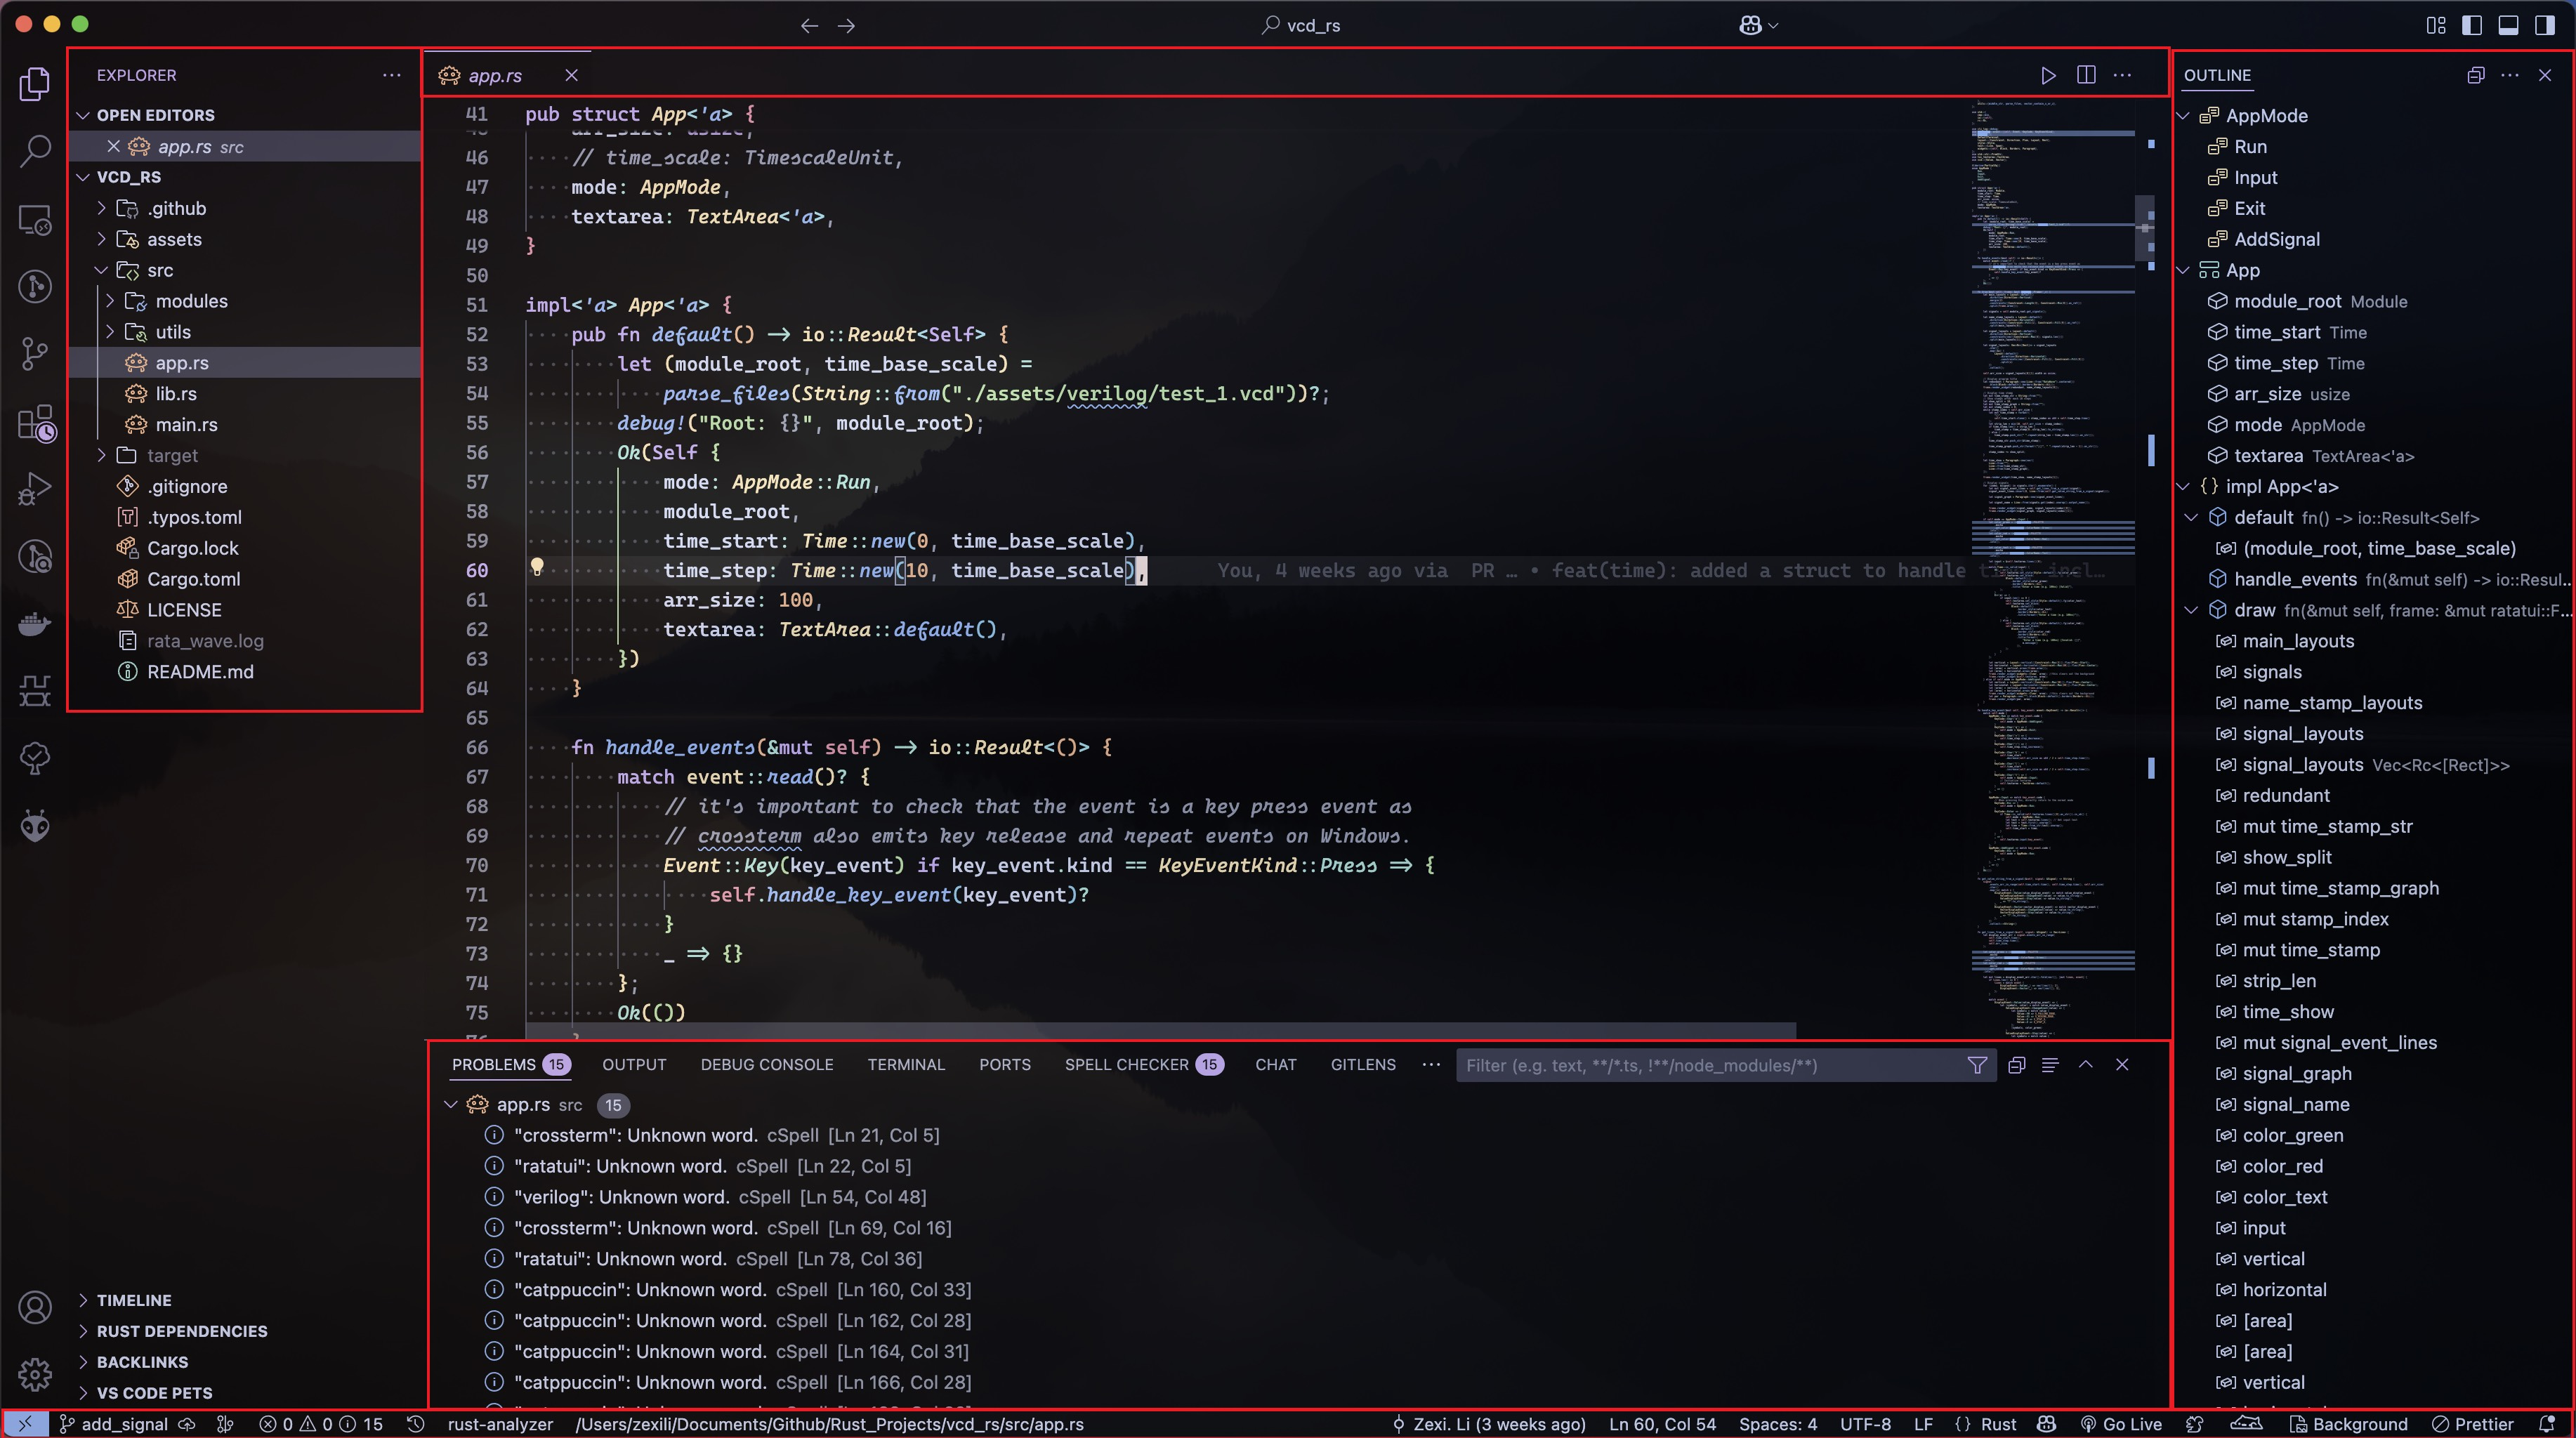
\includegraphics[width=0.9\linewidth]{./Figures/Vscode_interface_annotated.jpg}
      \end{figure}
    \end{column}
  \end{columns}

\end{frame}

\section{插件安装}

\subsection{gitsigns.nvim:显示文件git状态}
\begin{frame}[fragile]{\link{gitsigns.nvim}{https://github.com/lewis6991/gitsigns.nvim}:显示文件git状态}
  \begin{columns}
    \begin{column}{0.4\linewidth}
          \begin{lstlisting}[basicstyle=\tiny\ttfamily]
    -- ~/.config/nvim/lua/plugins/ui.lua

    {
      "lewis6991/gitsigns.nvim",
    },
        \end{lstlisting}
    \end{column}

    \begin{column}{0.6\linewidth}
      \begin{figure}[H]
        \centering
        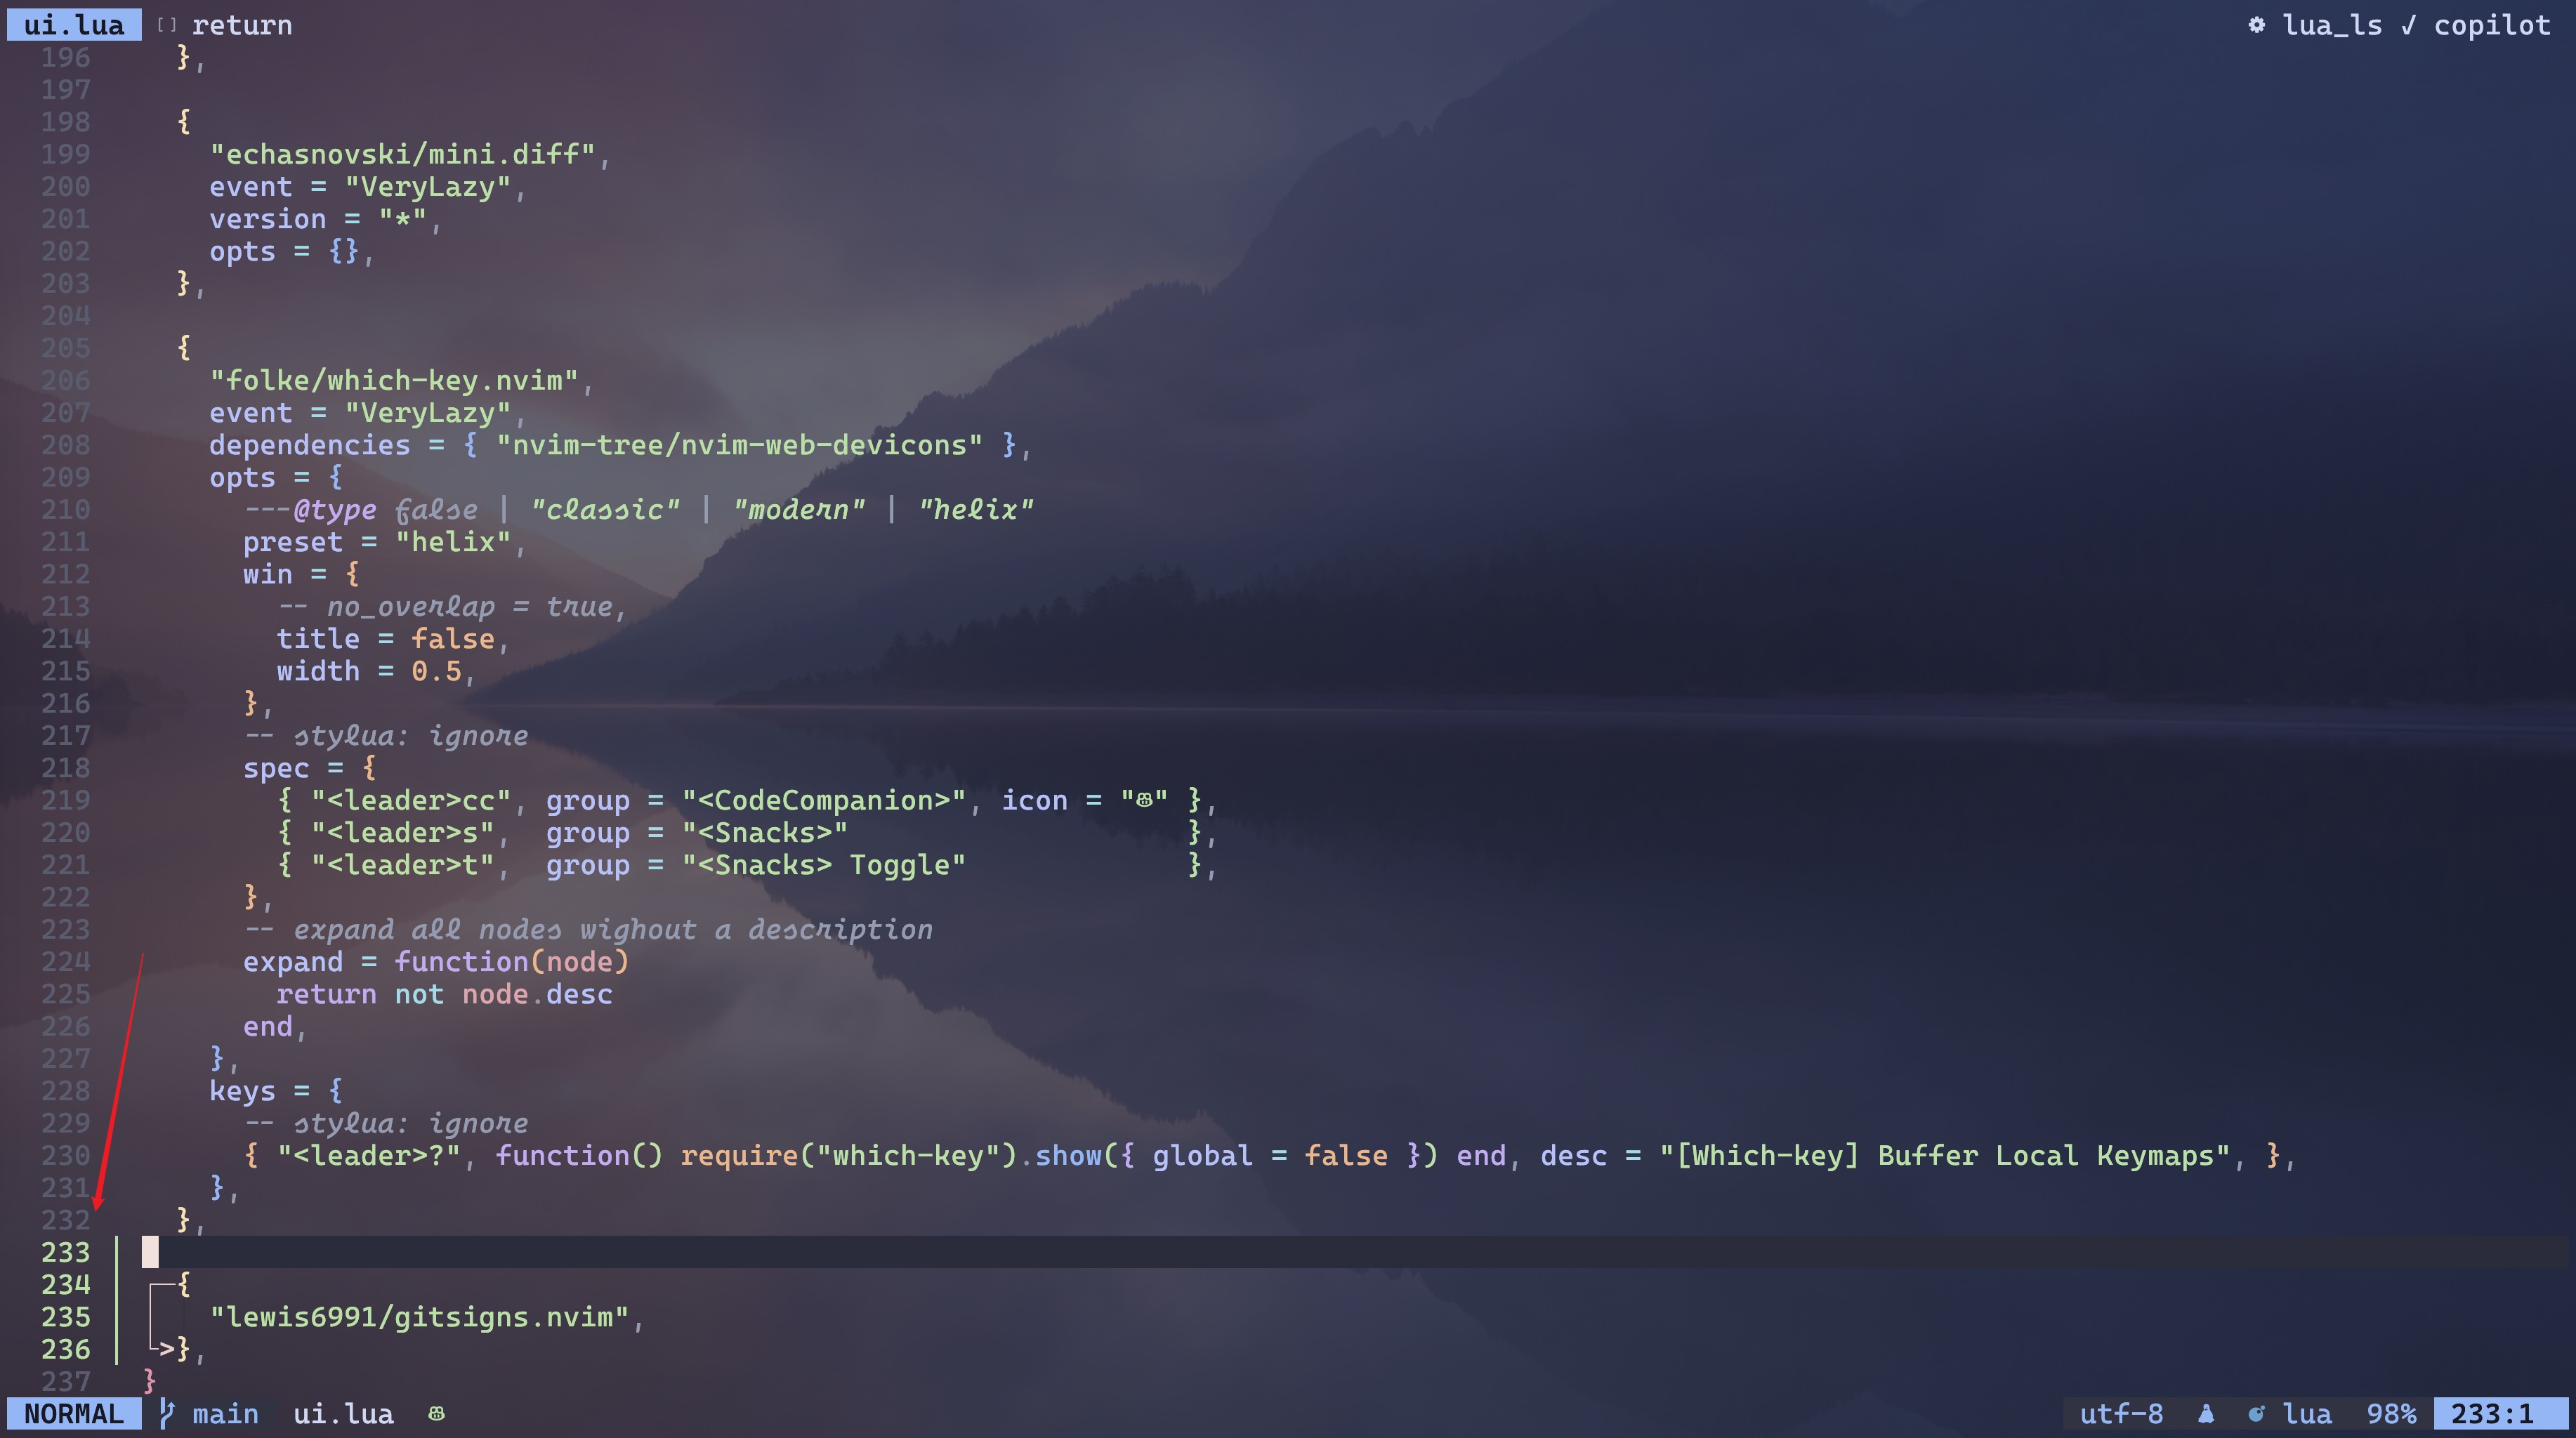
\includegraphics[width=\linewidth]{./Figures/Gitsigns_Finish.jpg}
        \caption{安装后的效果}%
      \end{figure}
    \end{column}
  \end{columns}
\end{frame}

\subsection{mini.diff:diff可视化}
\begin{frame}[fragile]{\link{mini.diff}{https://github.com/echasnovski/mini.diff}:diff可视化}
  \begin{columns}
    \begin{column}{0.4\linewidth}
        \begin{lstlisting}[basicstyle=\tiny\ttfamily]
    -- ~/.config/nvim/lua/plugins/ui.lua

    {
      "echasnovski/mini.diff",
      version = "*",
      opts = {},
    },
        \end{lstlisting}
    \end{column}

    \begin{column}{0.6\linewidth}
      \begin{figure}[H]
        \centering
        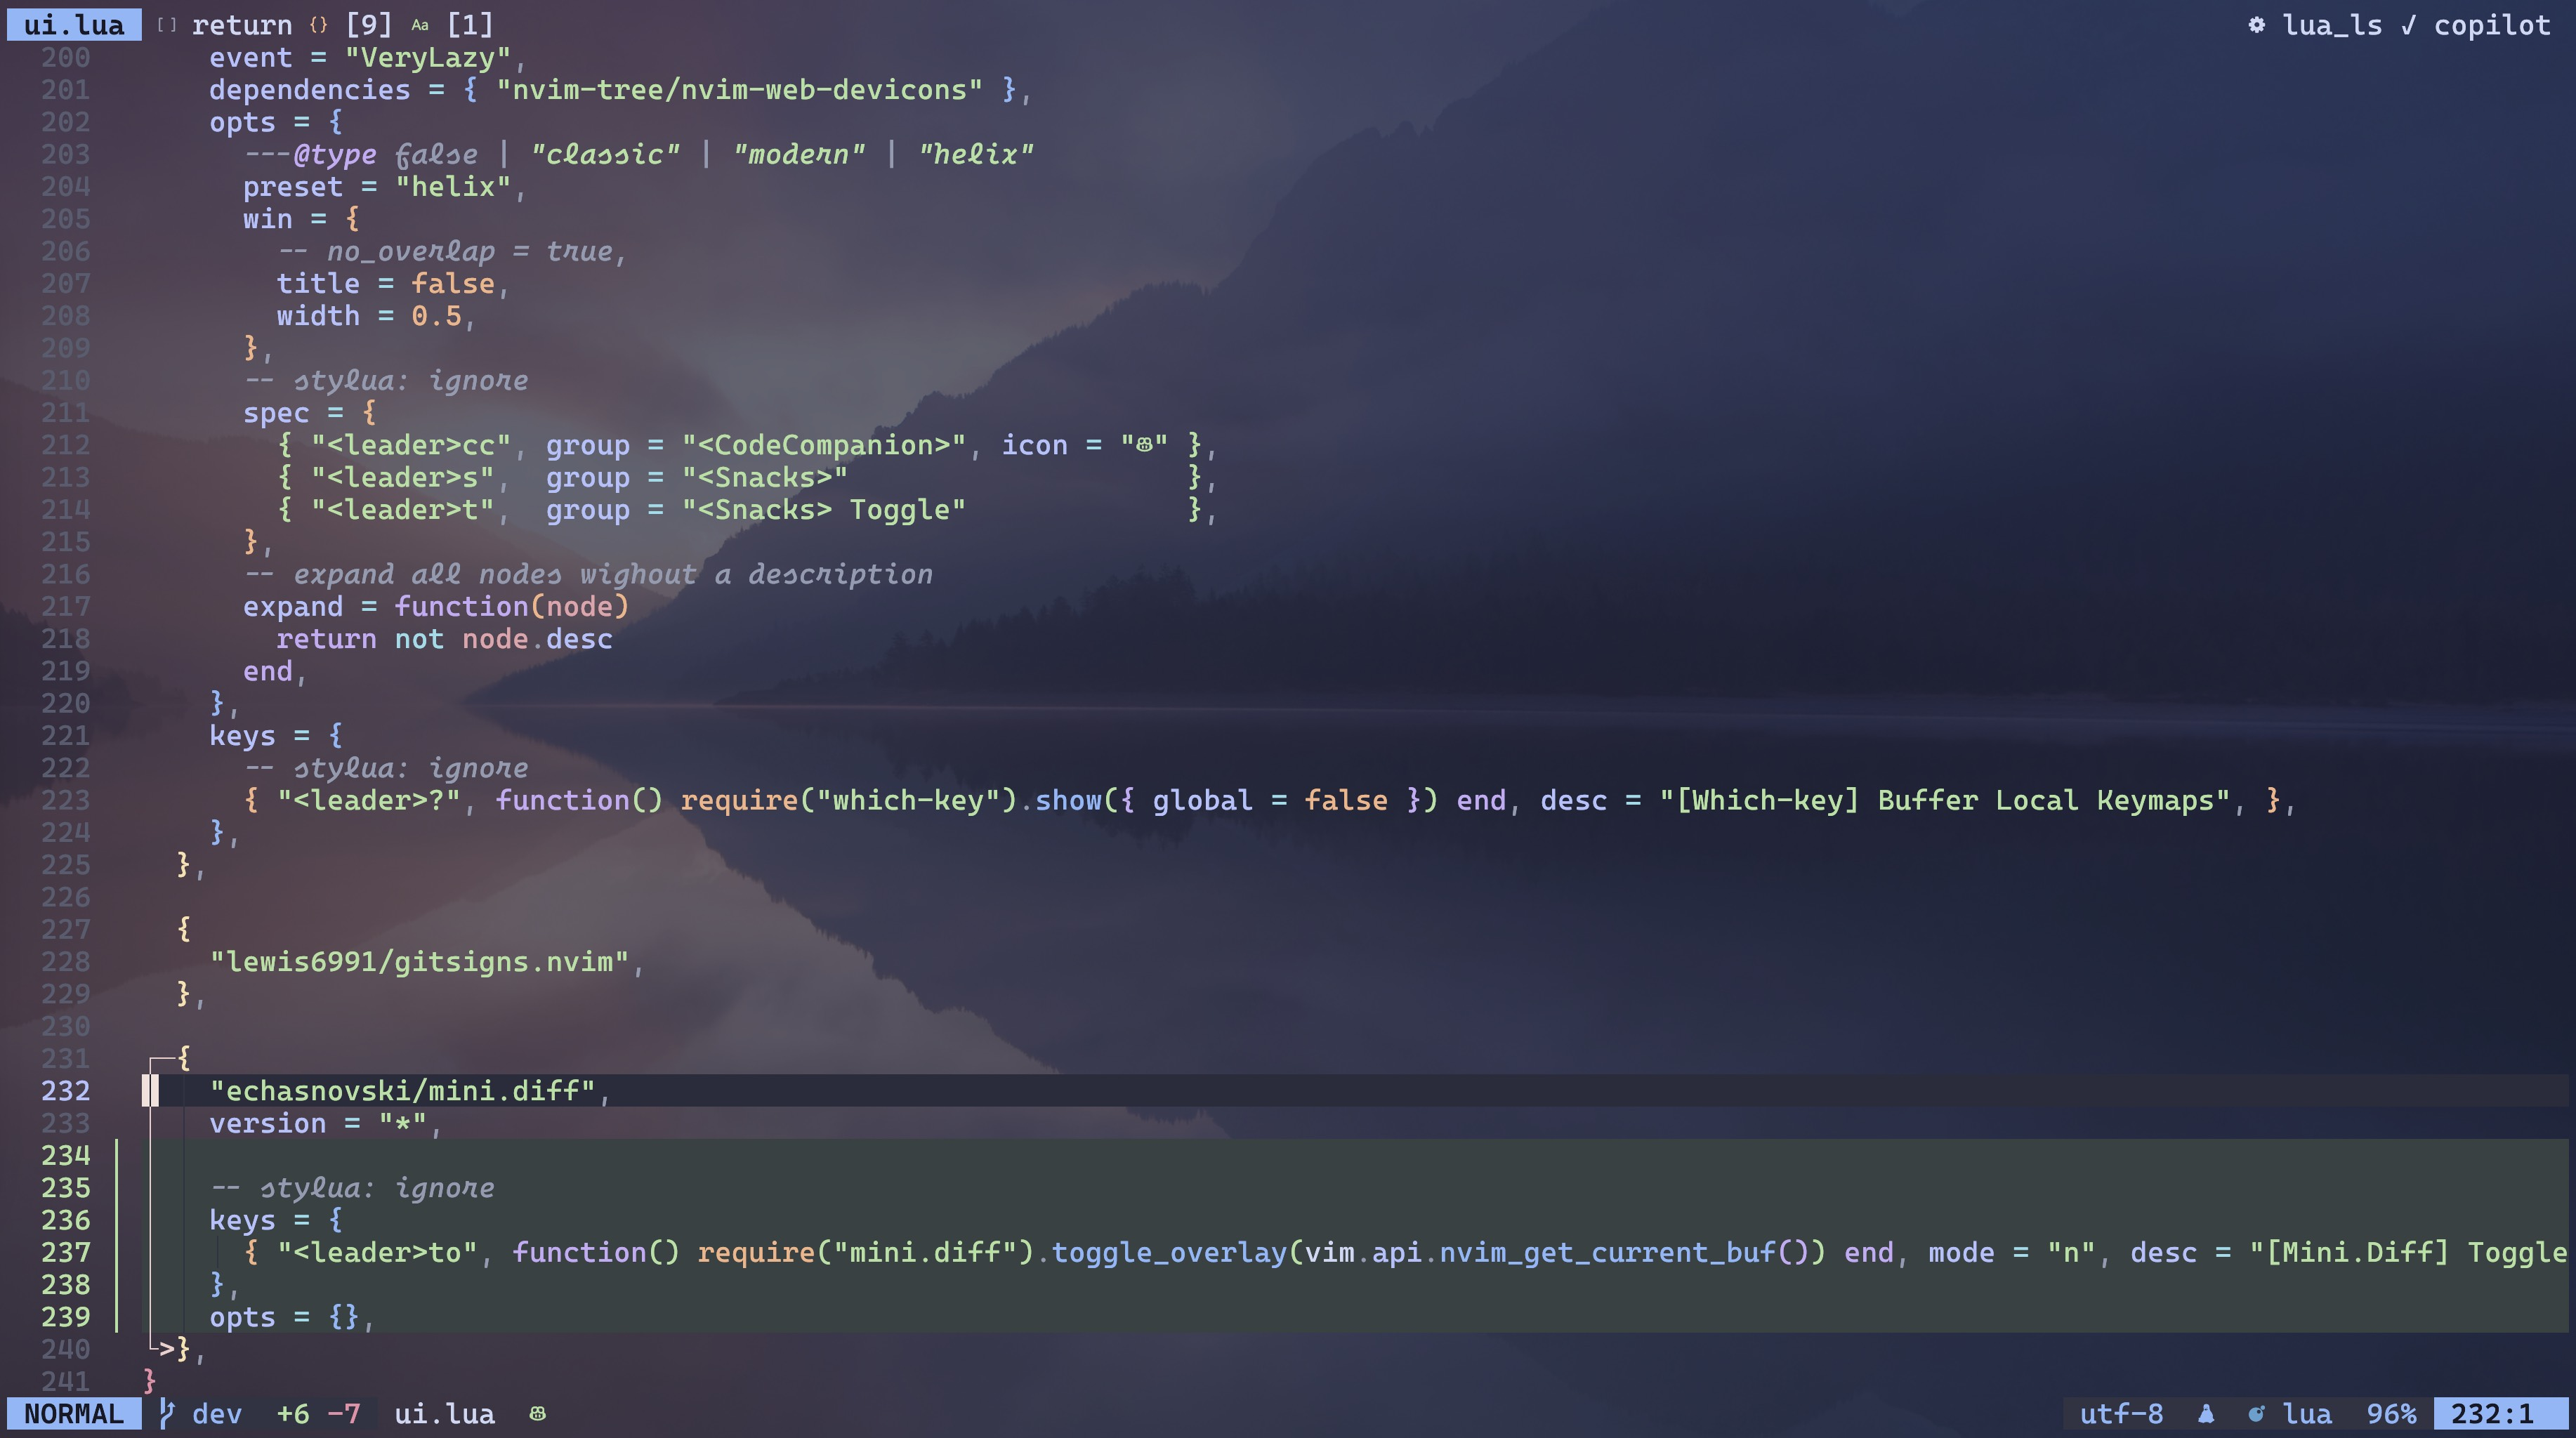
\includegraphics[width=\linewidth]{./Figures/MiniDiff_Finish.jpg}
        \caption{安装及配置后的效果}%
      \end{figure}
    \end{column}
  \end{columns}
\end{frame}

\subsection{nvim-scrollbar:滚动条}
\begin{frame}[fragile]{\link{nvim-scrollbar}{https://github.com/petertriho/nvim-scrollbar}:滚动条}
  \begin{columns}
    \begin{column}{0.4\linewidth}
        \begin{lstlisting}[basicstyle=\tiny\ttfamily]
    -- ~/.config/nvim/lua/plugins/ui.lua

    {
      "petertriho/nvim-scrollbar",
      opts = {},
    },
        \end{lstlisting}
    \end{column}

    \begin{column}{0.6\linewidth}
      \begin{figure}[H]
        \centering
        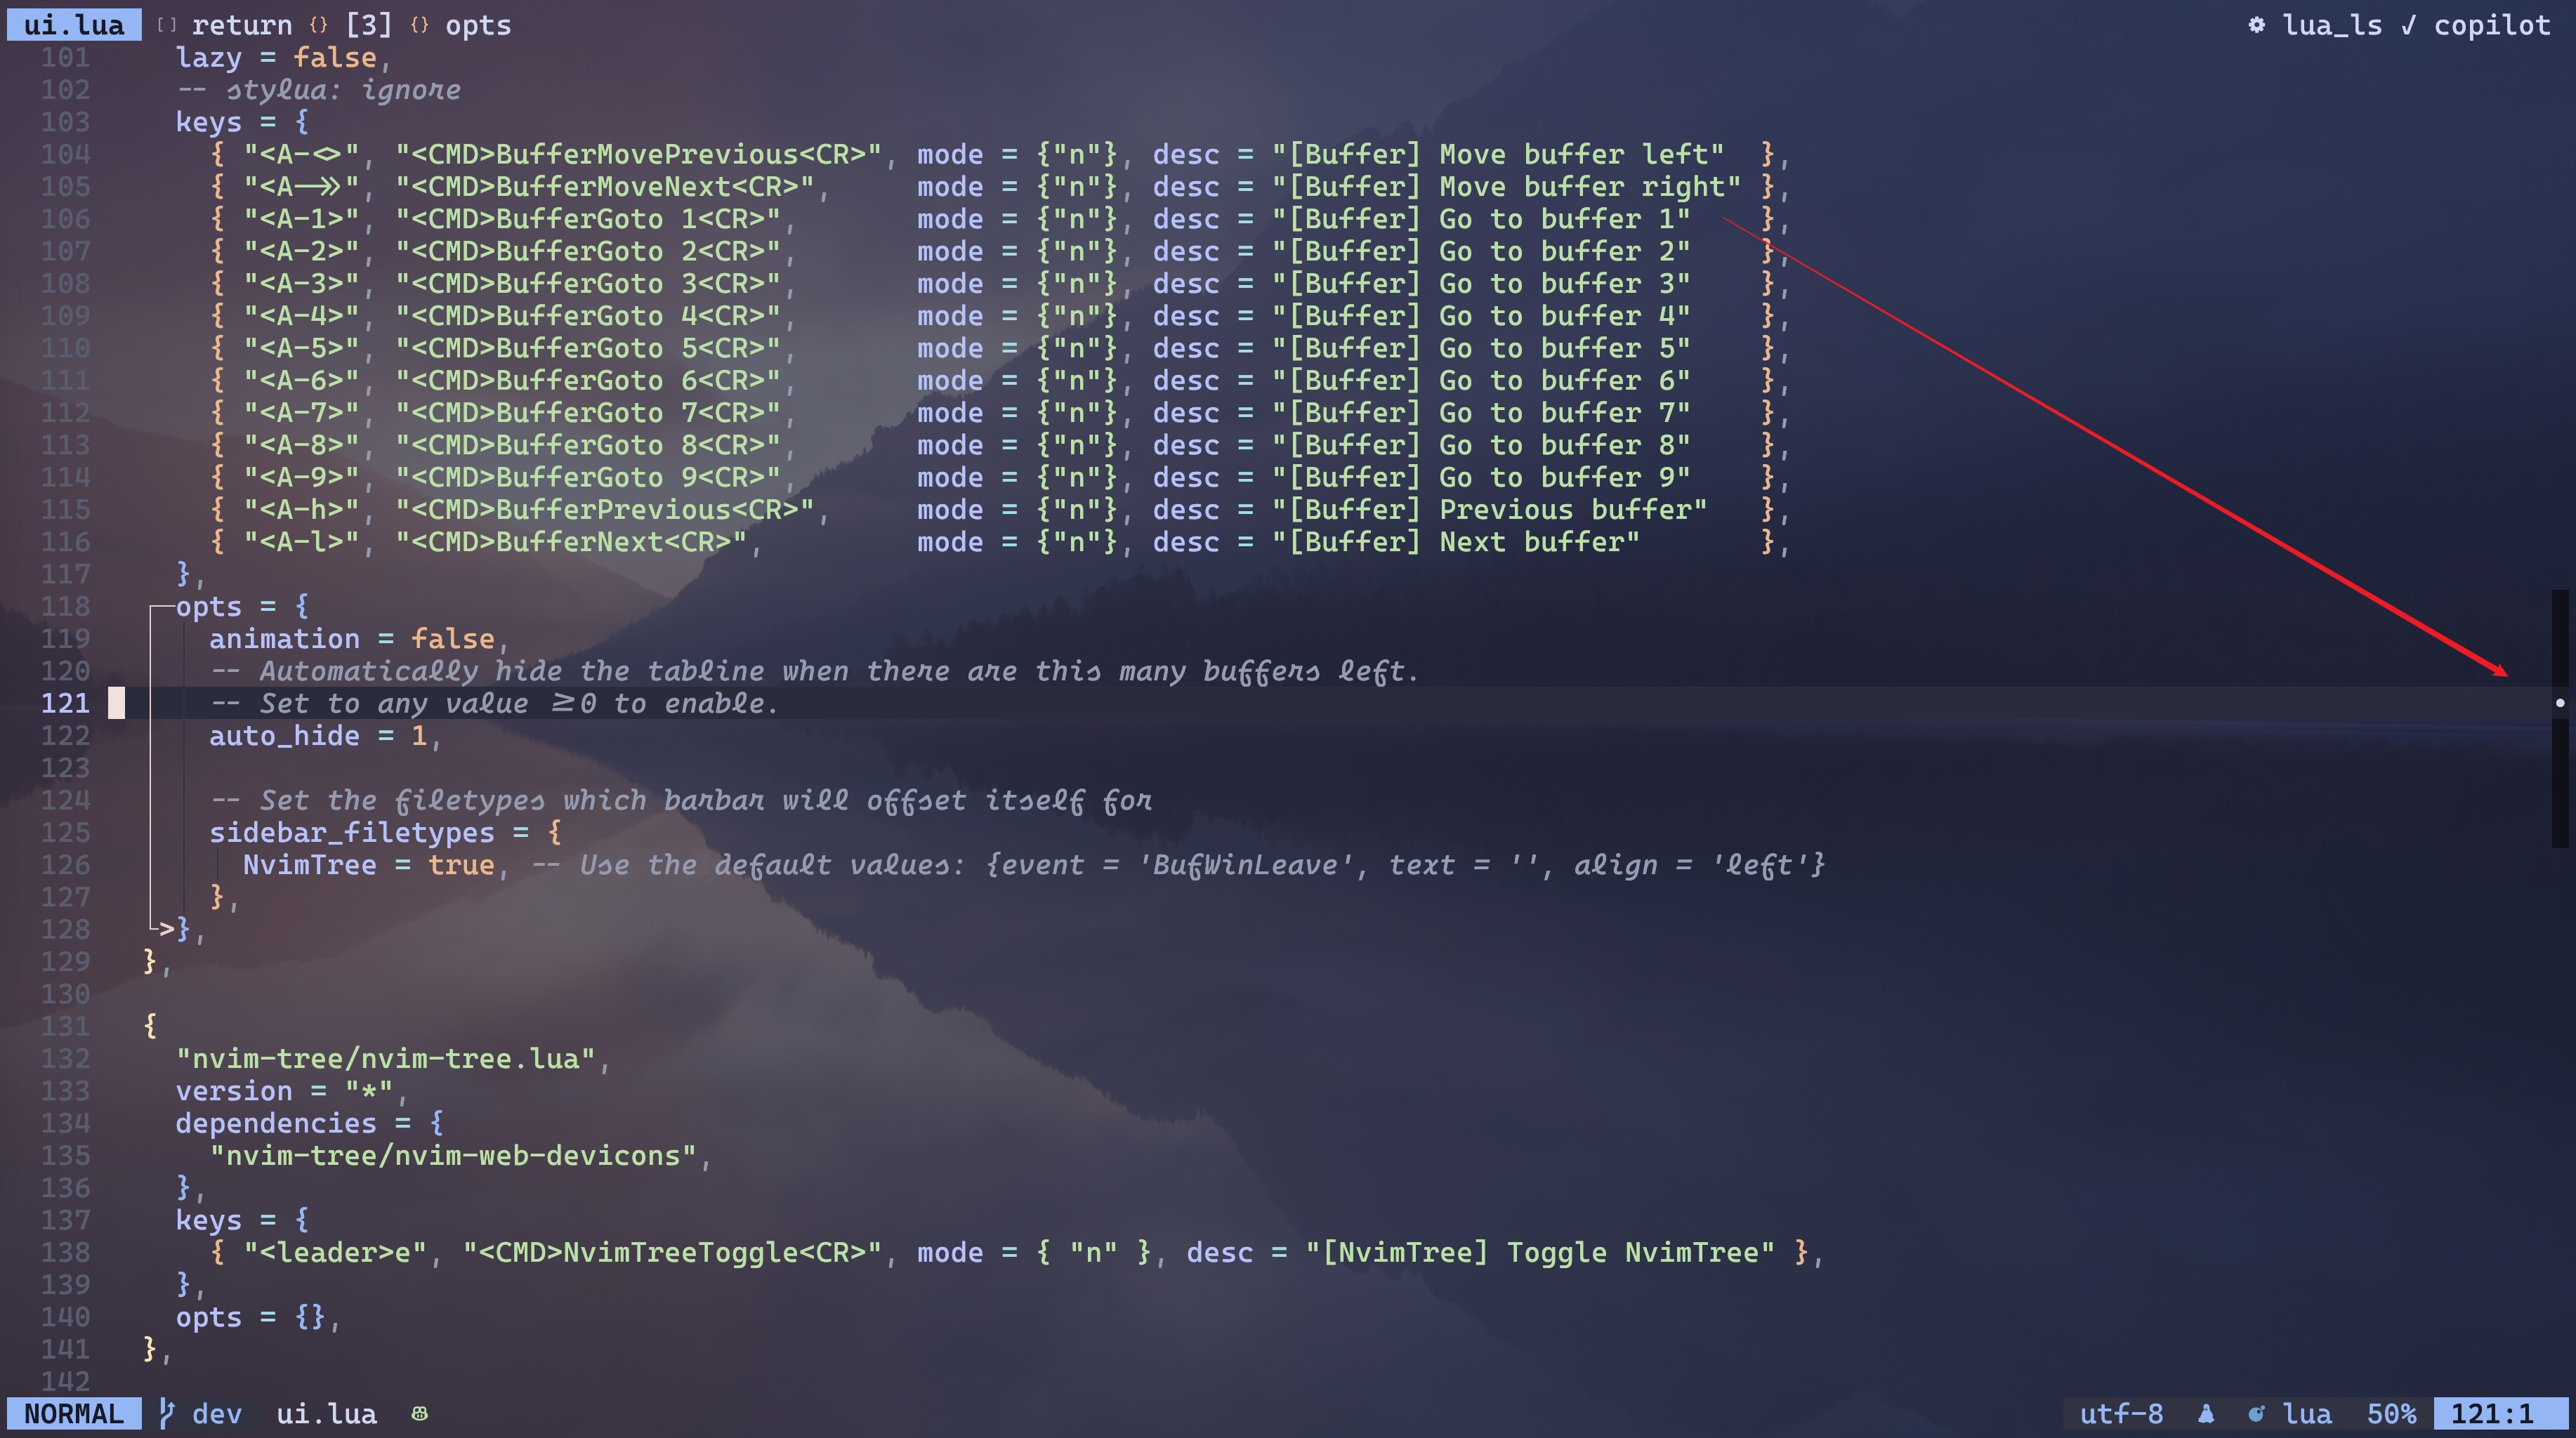
\includegraphics[width=\linewidth]{./Figures/Scrollbar_Finish.jpg}
        \caption{安装后的效果}%
      \end{figure}
    \end{column}
  \end{columns}
\end{frame}

\subsection{nvim-hlslens:显示搜索状态} % ChkTeX 19
\begin{frame}[fragile]{\link{nvim-hlslens}{https://github.com/kevinhwang91/nvim-hlslens}:显示搜索状态} % ChkTeX 19
  \begin{columns}
    \begin{column}{0.4\linewidth}
        \begin{lstlisting}[basicstyle=\tiny\ttfamily]
    -- ~/.config/nvim/lua/plugins/ui.lua

    {
      "kevinhwang91/nvim-hlslens",
      opts = {},
    },
        \end{lstlisting}
    \end{column}

    \begin{column}{0.6\linewidth}
      \begin{figure}[H]
        \centering
        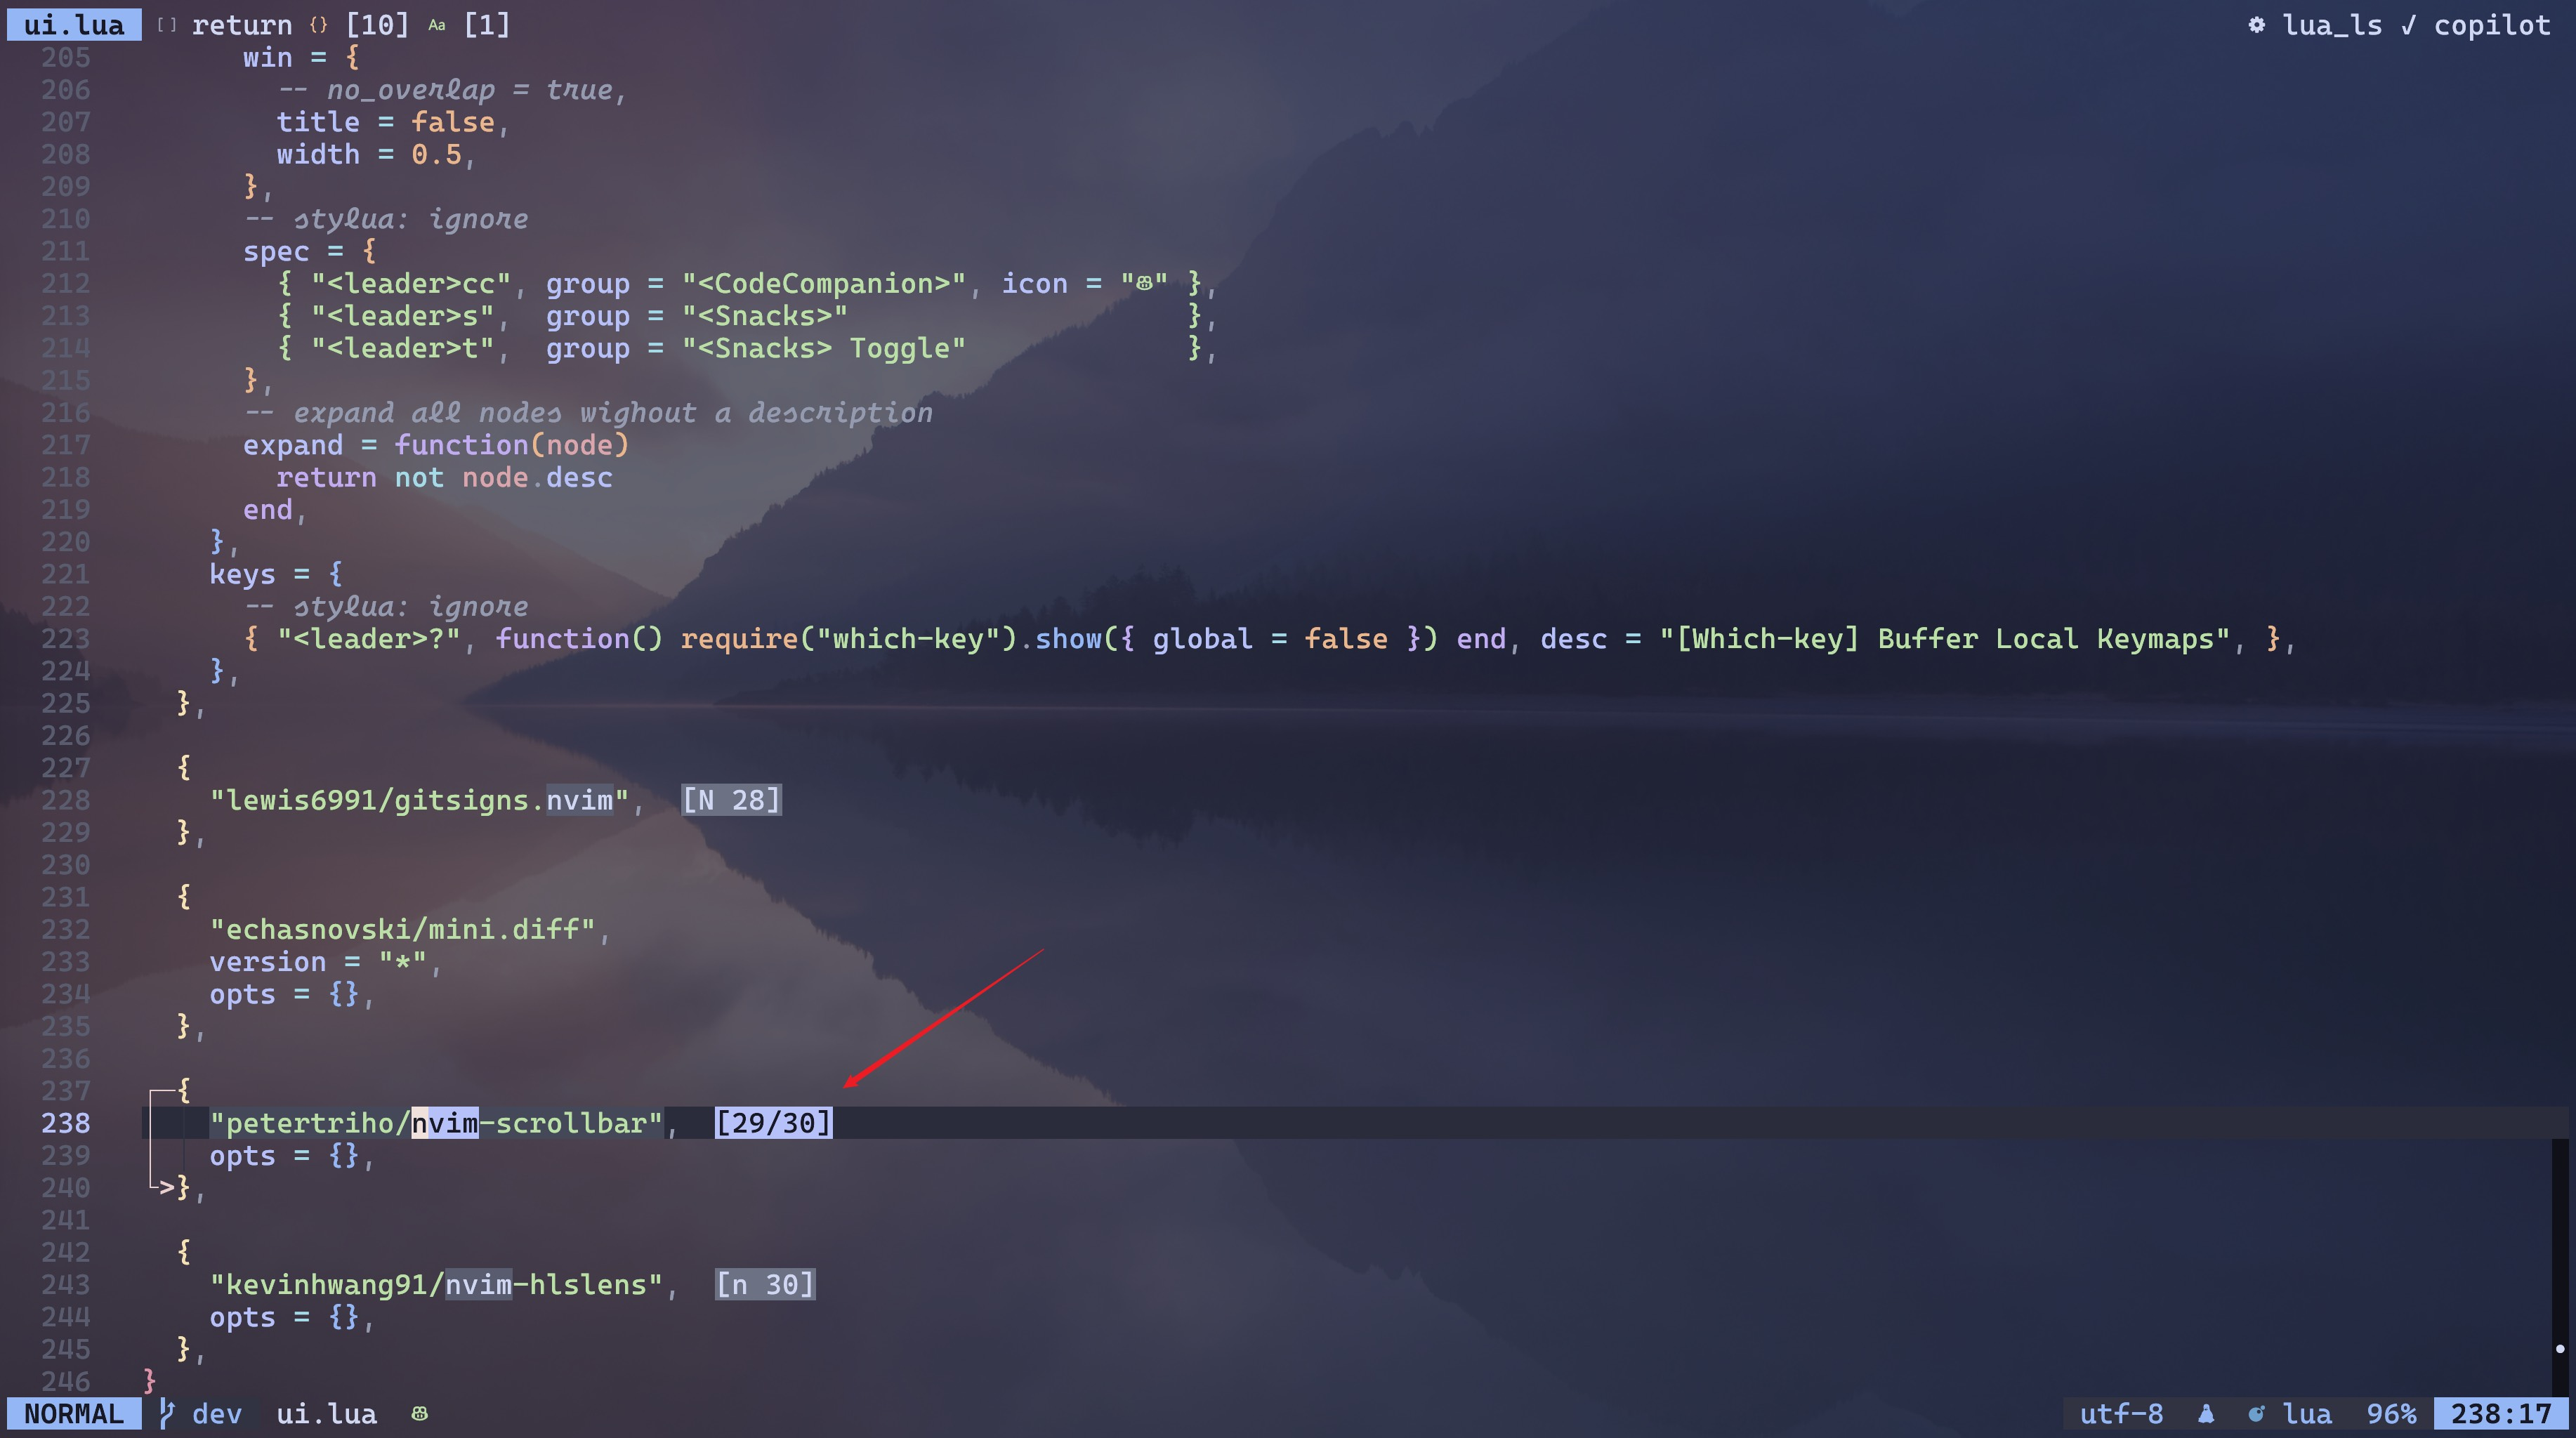
\includegraphics[width=\linewidth]{./Figures/Hlslens_Finish.jpg}
        \caption{安装后的效果}%
      \end{figure}
    \end{column}
  \end{columns}
\end{frame}

\subsection{nvim-colorizer.lua:颜色字符串高亮}
\begin{frame}[fragile]{\link{nvim-colorizer.lua}{https://github.com/norcalli/nvim-colorizer.lua}:颜色字符串高亮}
  \begin{columns}
    \begin{column}{0.4\linewidth}
        \begin{lstlisting}[basicstyle=\tiny\ttfamily]
    -- ~/.config/nvim/lua/plugins/ui.lua

    {
      "norcalli/nvim-colorizer.lua",
      config = function(_, _)
        require("colorizer").setup()
      end,
    },
        \end{lstlisting}
    \end{column}

    \begin{column}{0.6\linewidth}
      \begin{figure}[H]
        \centering
        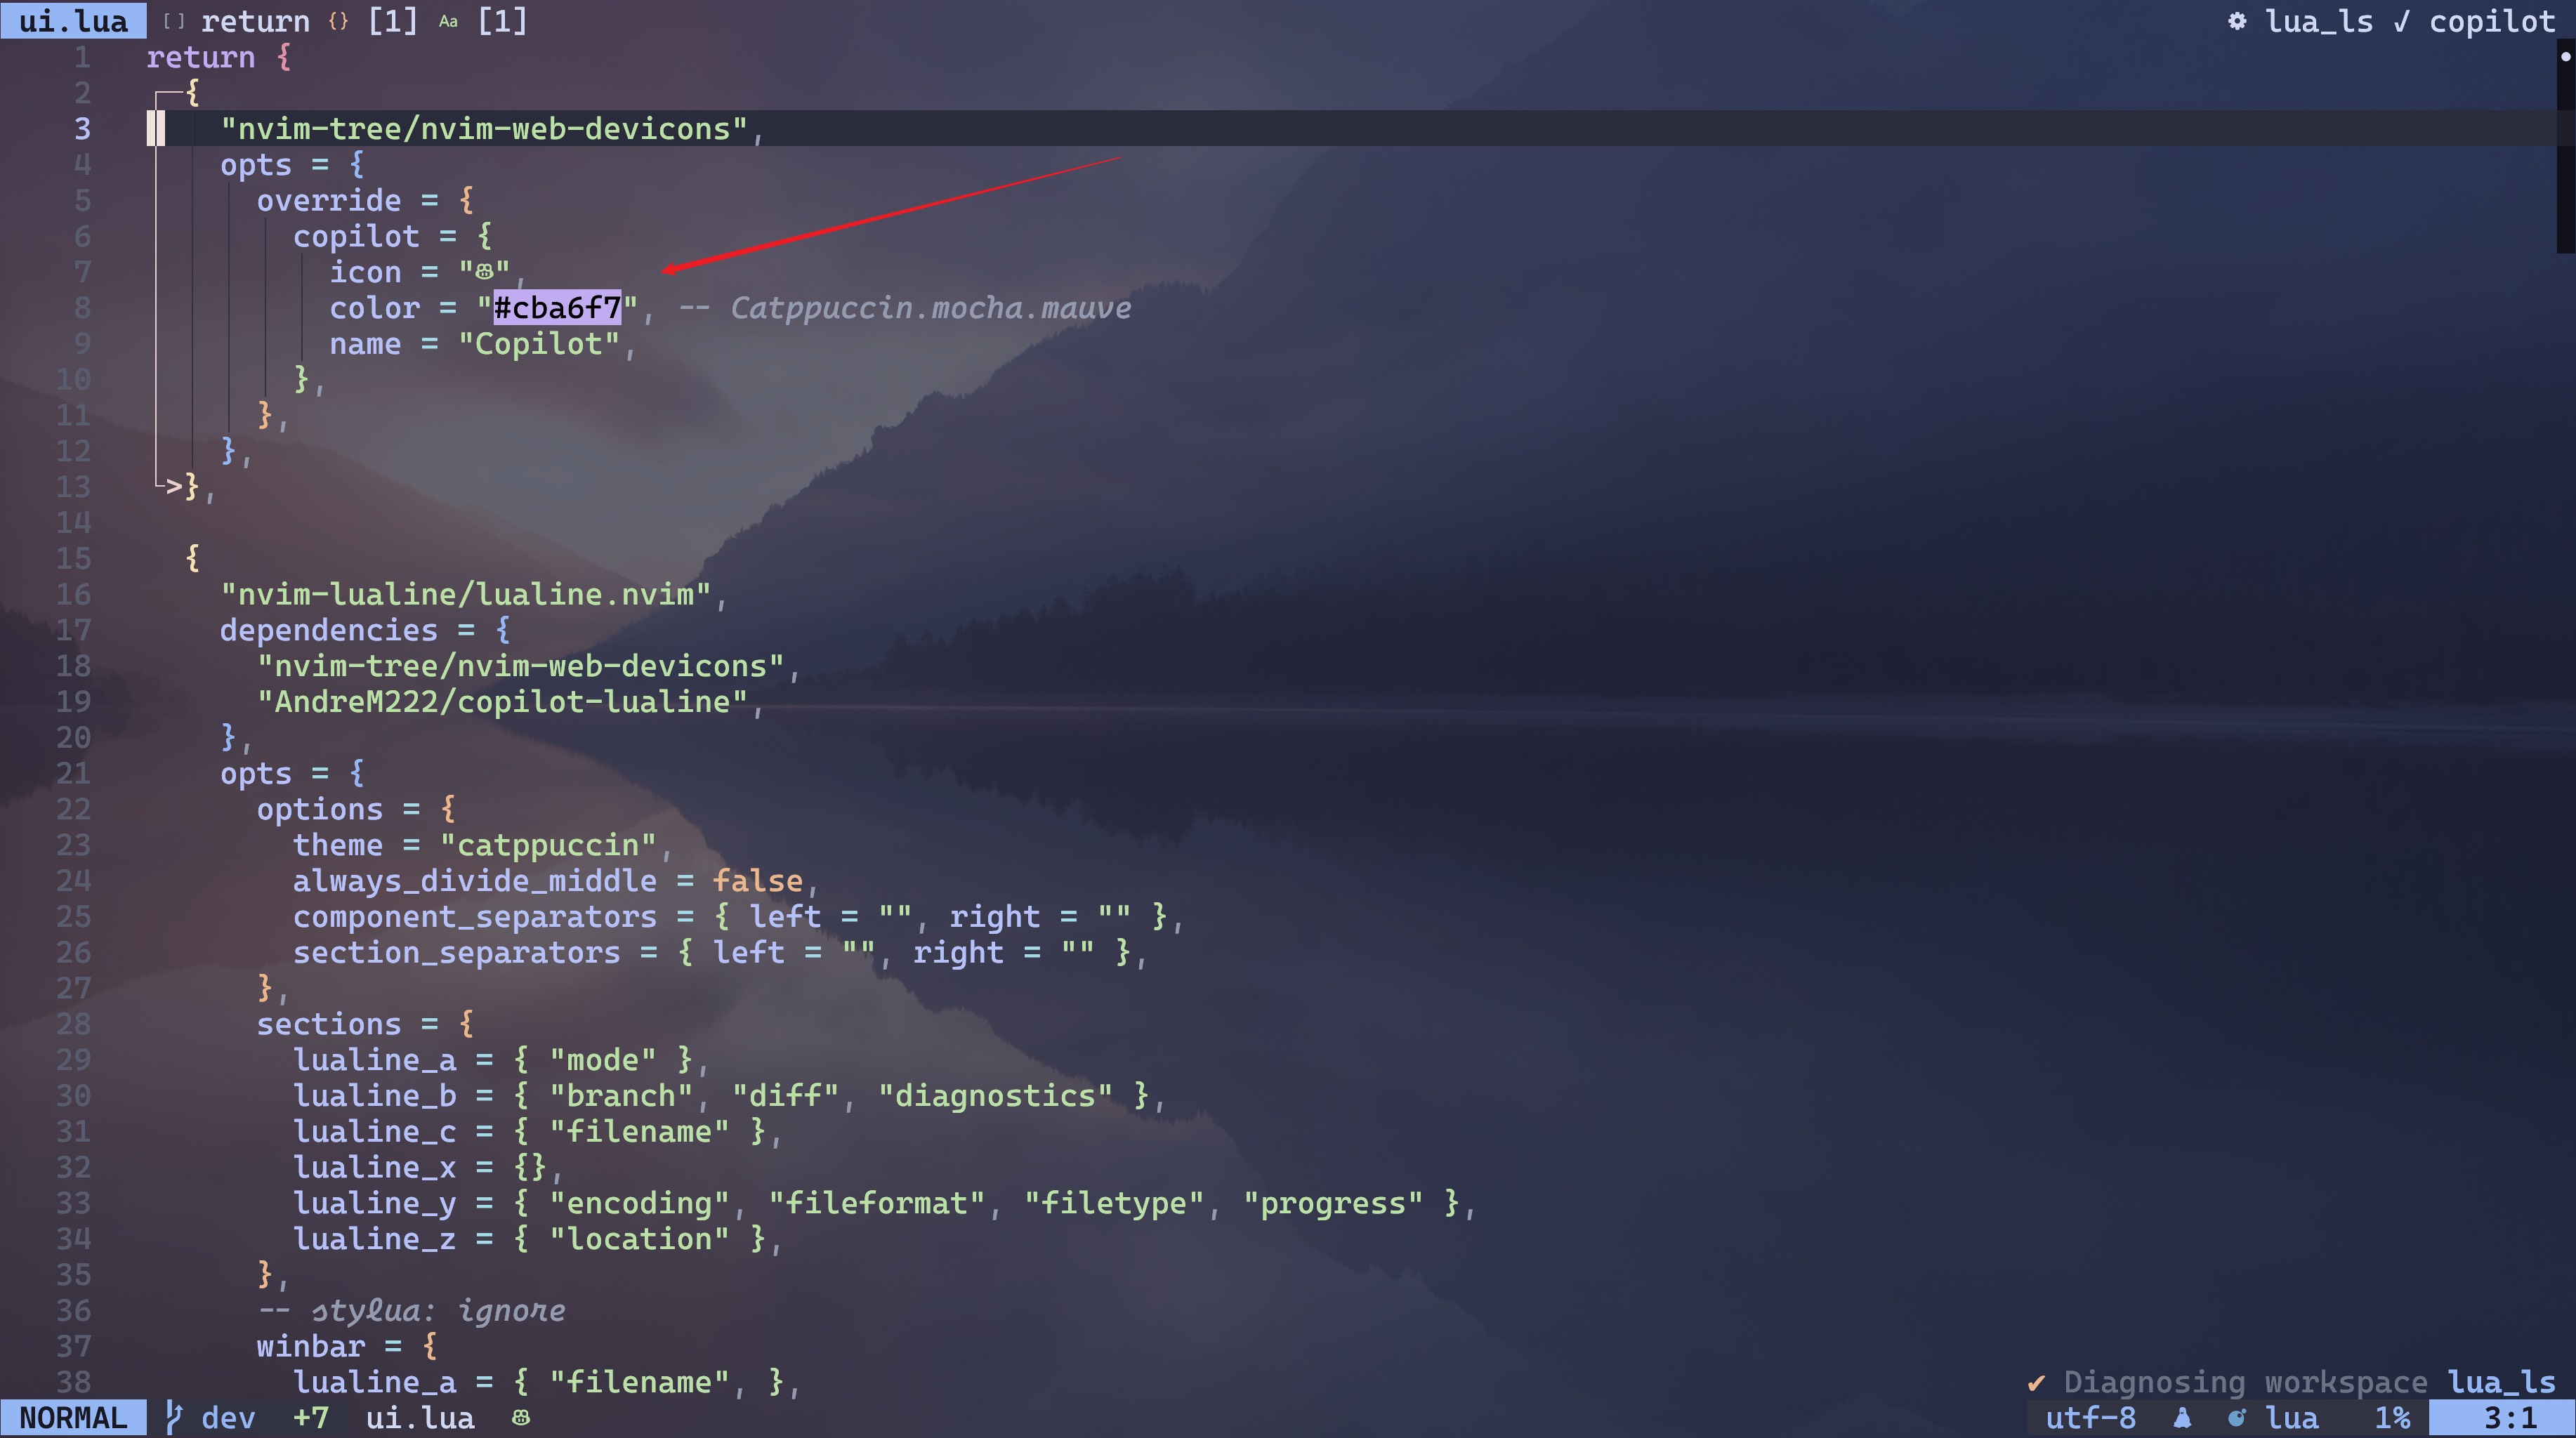
\includegraphics[width=\linewidth]{./Figures/Colorizer_Finish.jpg}
        \caption{安装后的效果}%
      \end{figure}
    \end{column}
  \end{columns}
\end{frame}

\subsection{showkeys:按键显示}
\begin{frame}[fragile]{\link{showkeys}{https://github.com/nvzone/showkeys}:按键显示}
  \begin{columns}
    \begin{column}{0.4\linewidth}
        \begin{lstlisting}[basicstyle=\tiny\ttfamily]
    -- ~/.config/nvim/lua/plugins/ui.lua

    {
      "nvzone/showkeys",
      cmd = "ShowkeysToggle",
      opts = {
        maxkeys = 5,
      },
    },
        \end{lstlisting}
    \end{column}

    \begin{column}{0.6\linewidth}
      \begin{figure}[H]
        \centering
        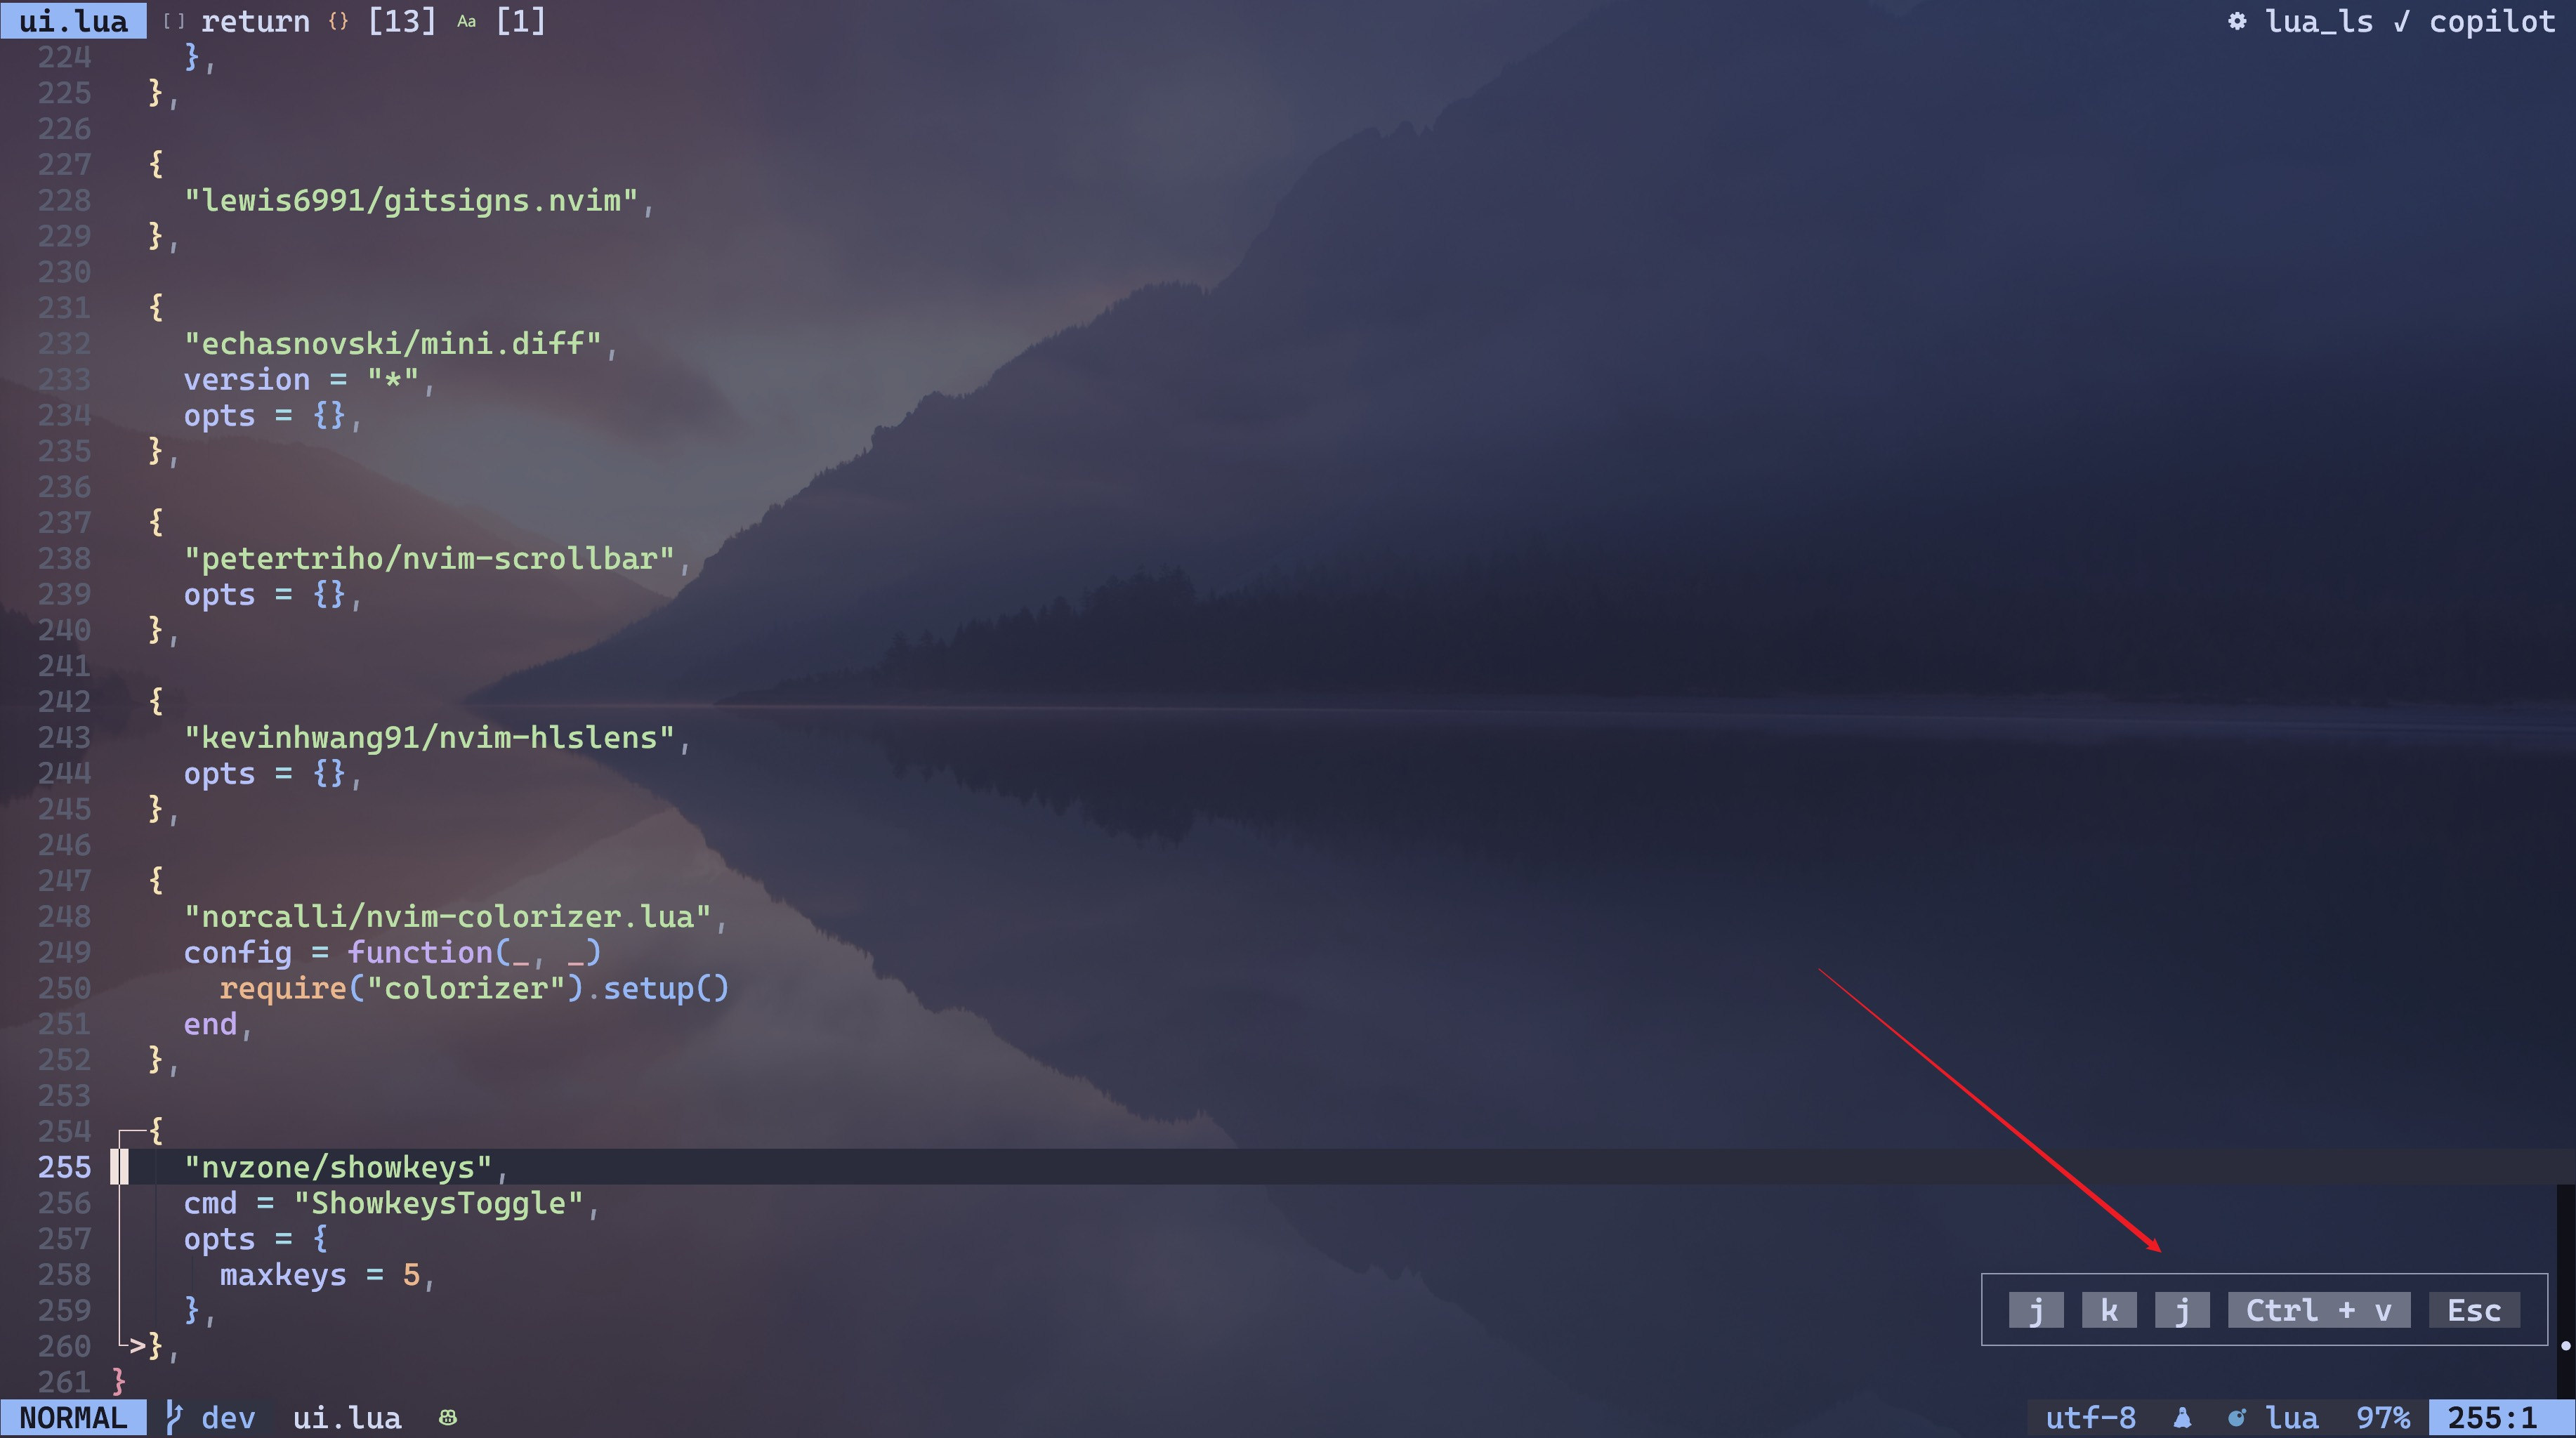
\includegraphics[width=\linewidth]{./Figures/Showkeys_Finish.jpg}
        \caption{安装后的效果}%
      \end{figure}
    \end{column}
  \end{columns}
\end{frame}

\subsection{nvim-lightbulb:可用code actions提示}
\begin{frame}[fragile]{\link{nvim-lightbulb}{https://github.com/kosayoda/nvim-lightbulb}:可用code actions提示}
  \begin{columns}
    \begin{column}{0.4\linewidth}
        \begin{lstlisting}[basicstyle=\tiny\ttfamily]
    -- ~/.config/nvim/lua/plugins/ui.lua

    {
      "kosayoda/nvim-lightbulb",
    },
        \end{lstlisting}
    \end{column}

    \begin{column}{0.6\linewidth}
      \begin{figure}[H]
        \centering
        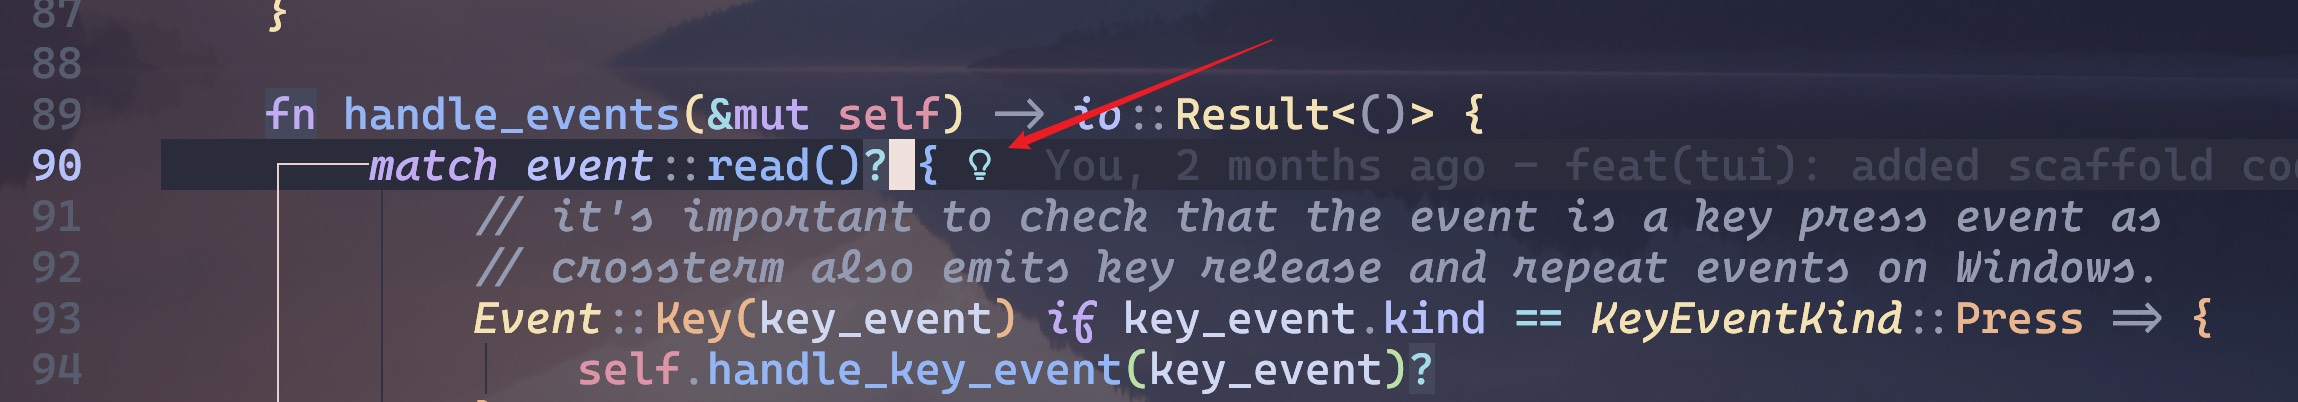
\includegraphics[width=\linewidth]{./Figures/Lightbulb_Finish.jpg}
        \caption{安装及配置后的效果}%
      \end{figure}
    \end{column}
  \end{columns}
\end{frame}

\subsection{tiny-code-action.nvim:Code action可视化}
\begin{frame}[fragile]{\link{tiny-code-action.nvim}{https://github.com/rachartier/tiny-code-action.nvim}:Code action可视化}
  \begin{columns}
    \begin{column}{0.4\linewidth}
        \begin{lstlisting}[basicstyle=\tiny\ttfamily]
    -- ~/.config/nvim/lua/plugins/ui.lua

    {
      "rachartier/tiny-code-action.nvim",
      dependencies = {
        { "nvim-lua/plenary.nvim" },
        {
          "folke/snacks.nvim",
          opts = {
            terminal = {},
          },
        },
      },
      event = "LspAttach",
      opts = {},
    },
        \end{lstlisting}
    \end{column}

    \begin{column}{0.6\linewidth}
      \begin{figure}[H]
        \centering
        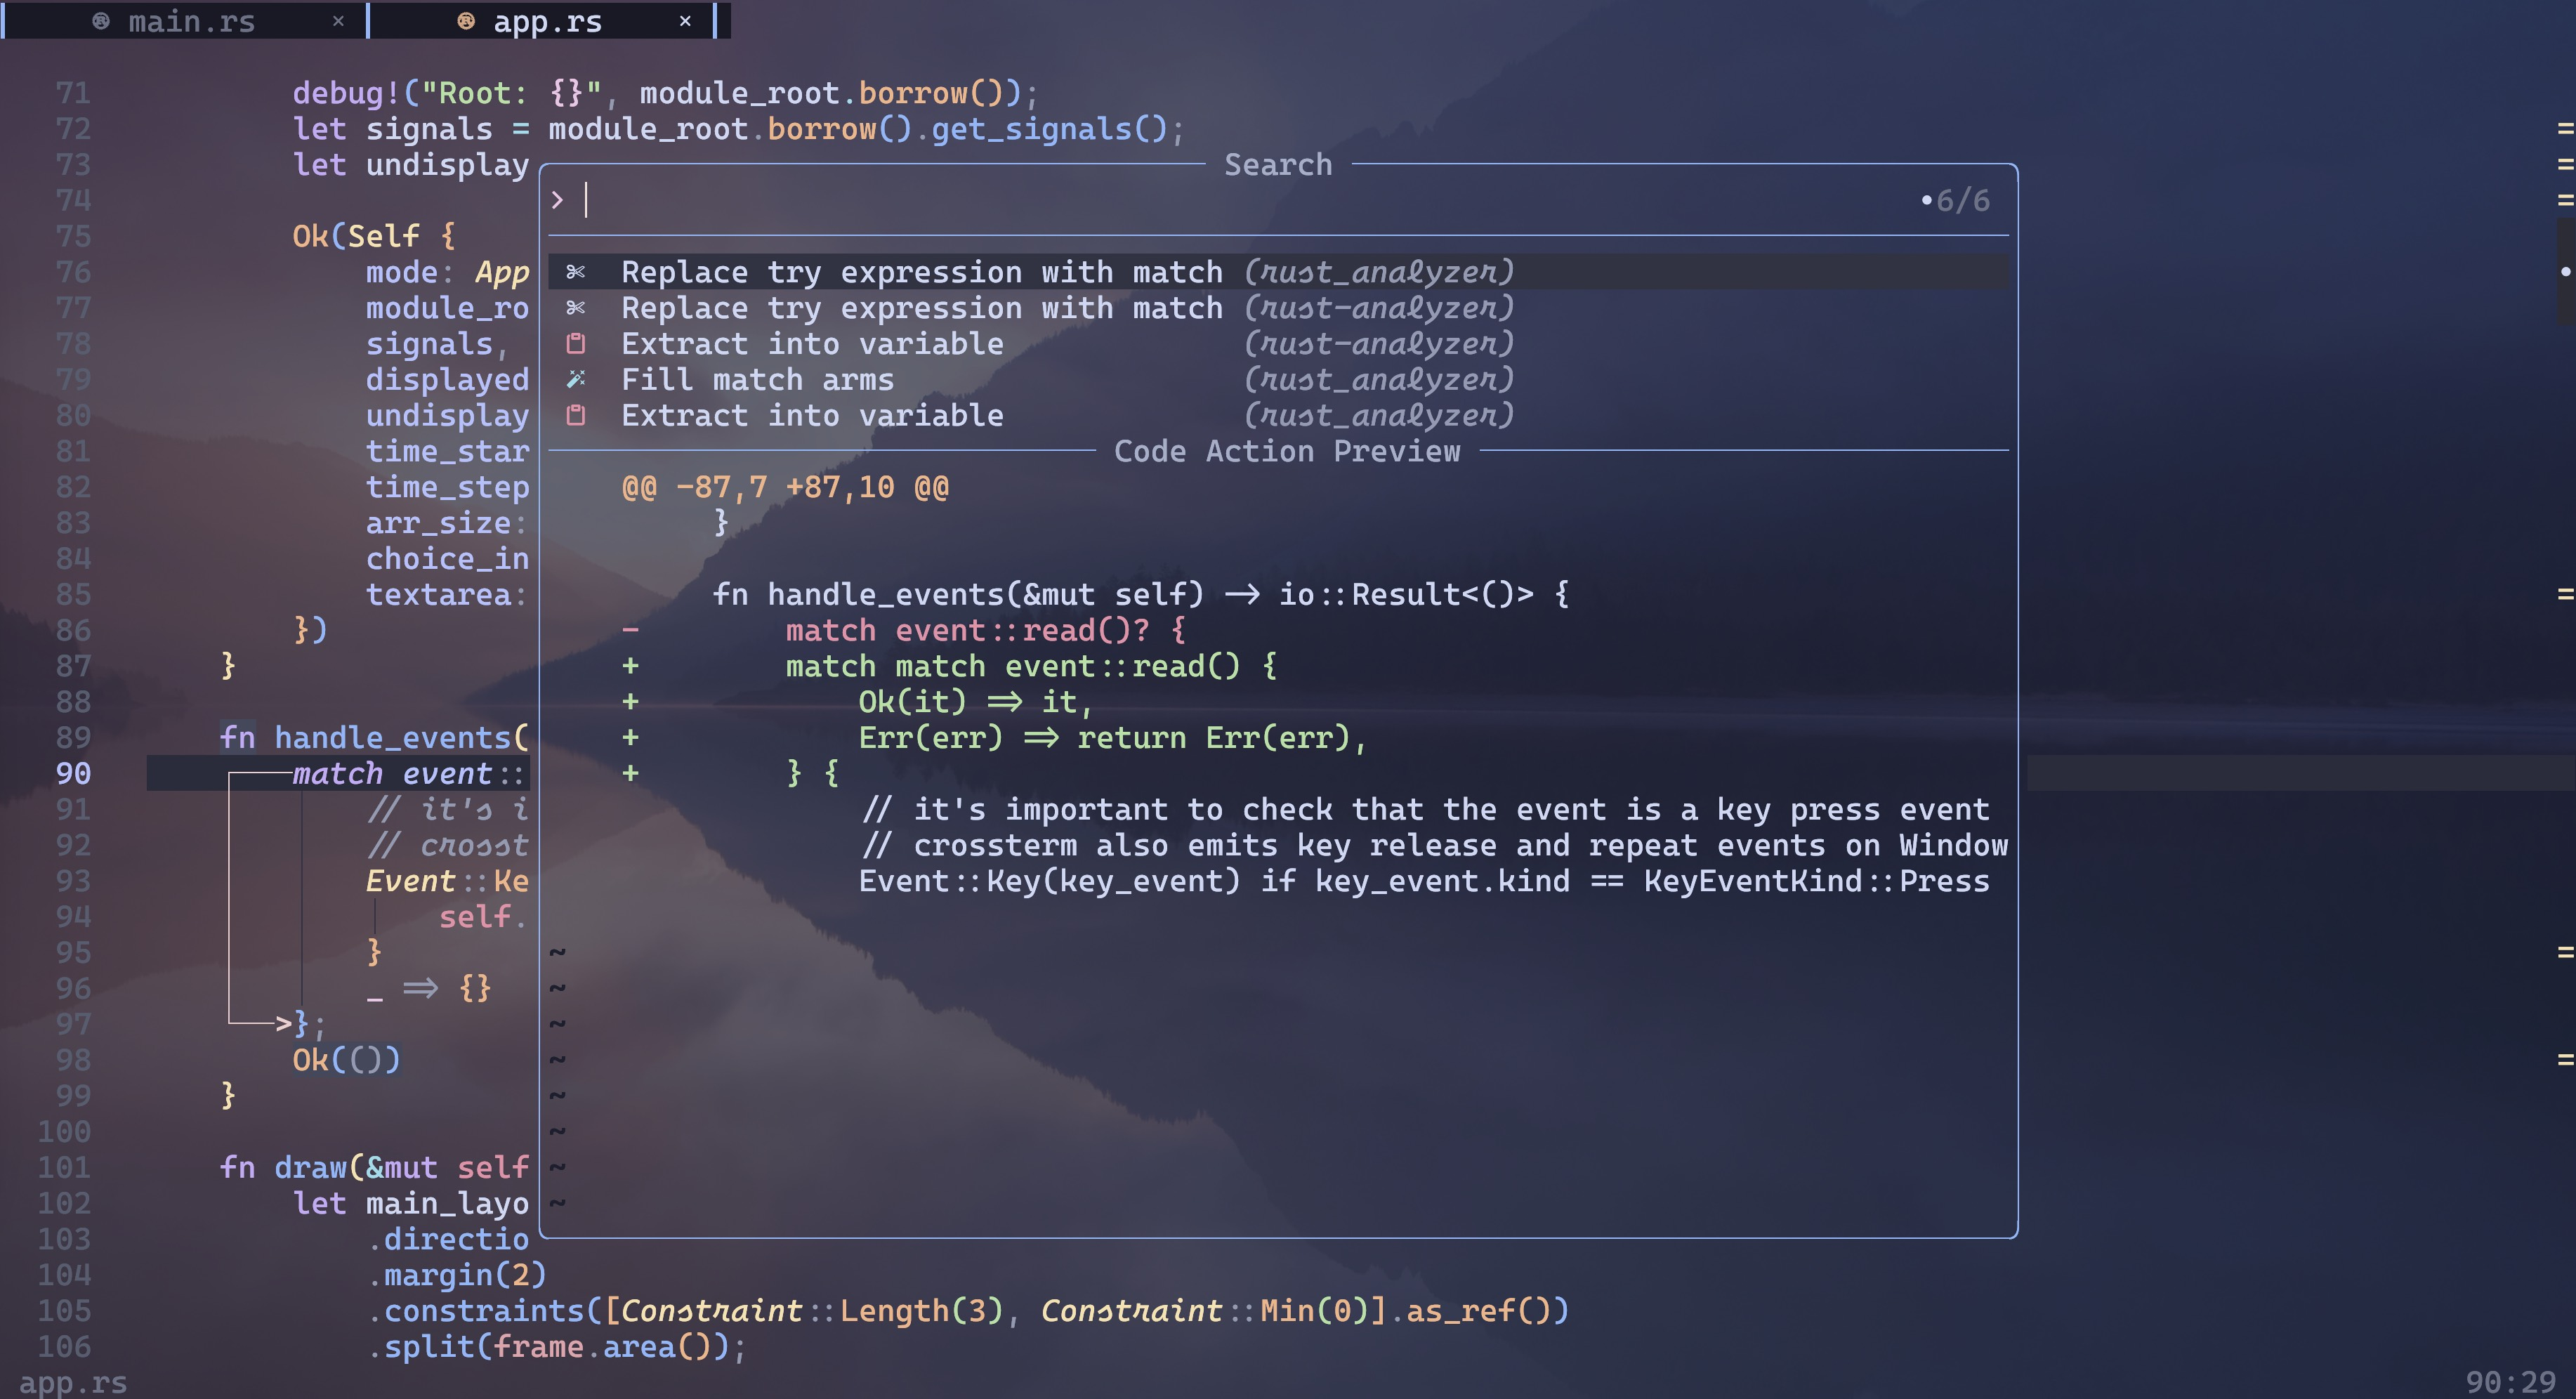
\includegraphics[width=\linewidth]{./Figures/TinyCodeAction_Finish.jpg}
        \caption{安装及配置后的效果}%
      \end{figure}
    \end{column}
  \end{columns}
\end{frame}

\subsection{nvim-ufo:代码折叠}
\begin{frame}[fragile]{\link{nvim-ufo}{https://github.com/kevinhwang91/nvim-ufo}:代码折叠}
  \begin{columns}
    \begin{column}{0.4\linewidth}
        \begin{lstlisting}[basicstyle=\tiny\ttfamily]
    -- ~/.config/nvim/lua/plugins/ui.lua

    {
      "kevinhwang91/nvim-ufo",
      dependencies = { "kevinhwang91/promise-async" },
      opts = {
        provider_selector = function(_, _, _)
          return { "treesitter", "indent" }
        end,
      },
      init = function()
        vim.o.foldenable = true
        vim.o.foldcolumn = "0"
        vim.o.foldlevel = 99
        vim.o.foldlevelstart = 99
        vim.opt.fillchars = {
          fold = " ",
          foldopen = "▾",
          foldsep = "│",
          foldclose = "▸",
        }
      end,
    },
        \end{lstlisting}
    \end{column}

    \begin{column}{0.6\linewidth}
      \begin{figure}[H]
        \centering
        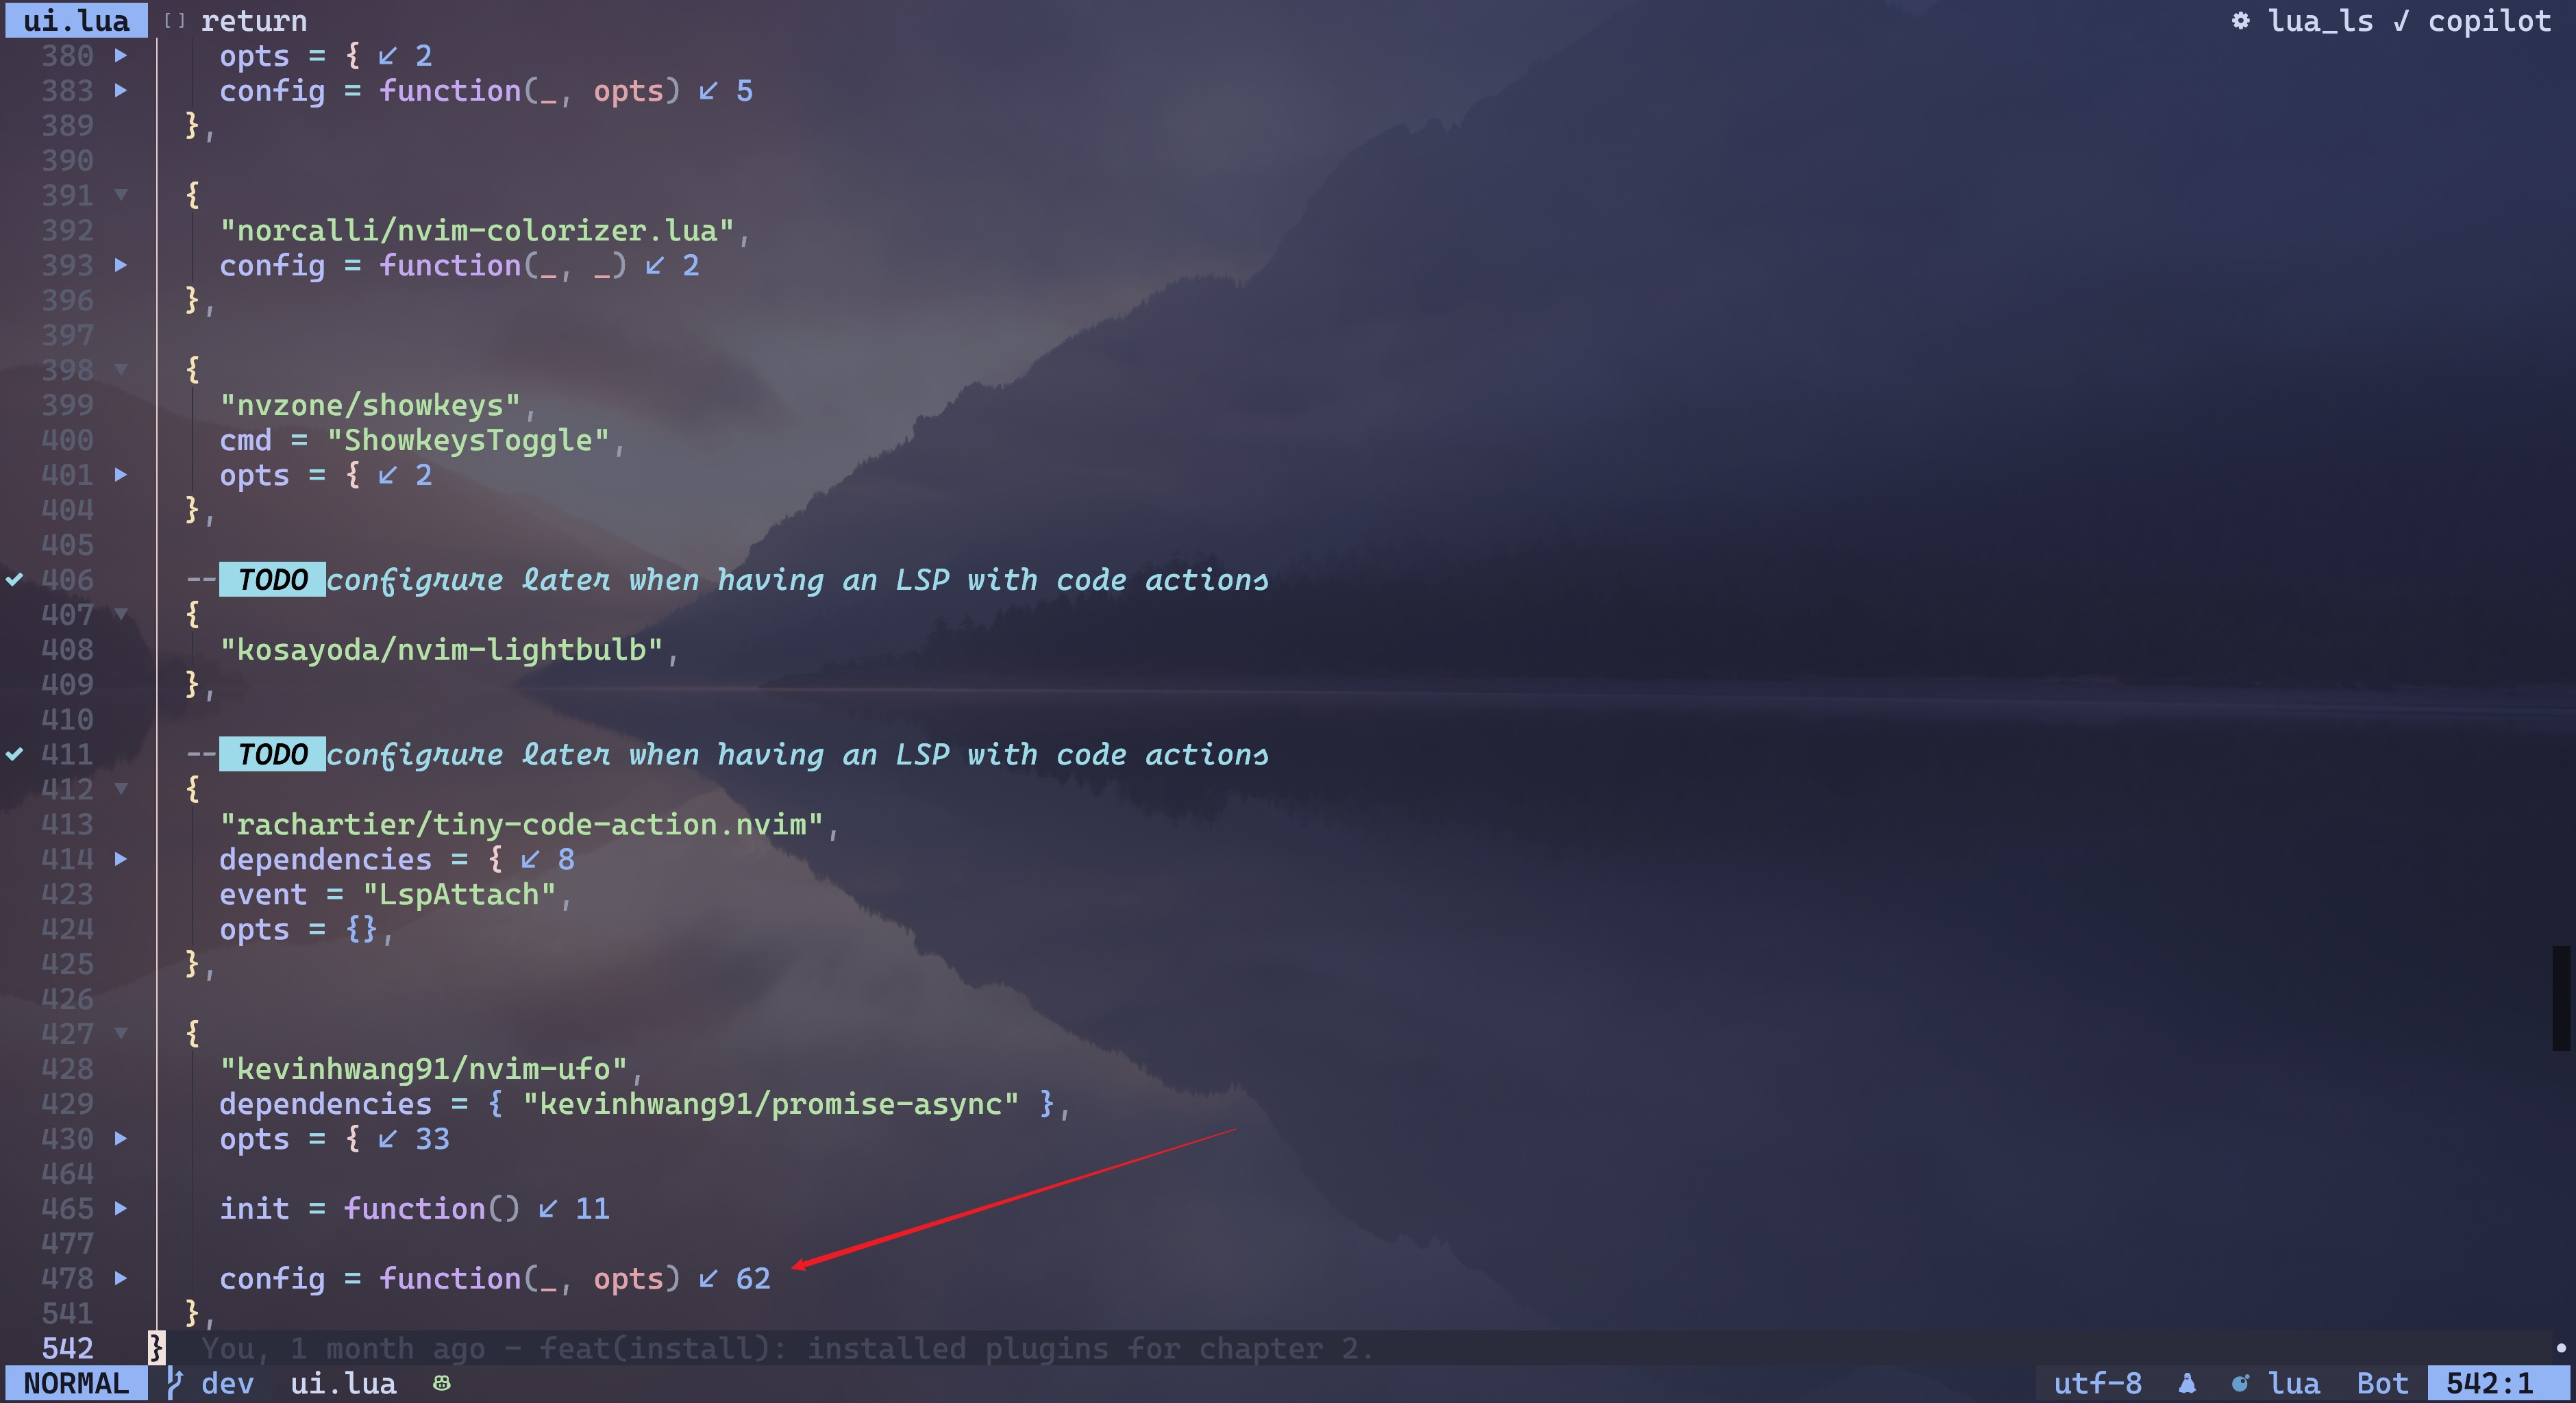
\includegraphics[width=\linewidth]{./Figures/Ufo_Finish.jpg}
        \caption{安装及配置后的效果}%
      \end{figure}
    \end{column}
  \end{columns}
\end{frame}

\section{插件配置}

\begin{frame}{插件配置}
  见演示
  \begin{itemize}
    \item 本节所有插件:\lstinline[language={},style=path]{\~/.config/nvim/lua/plugins/ui.lua}
  \end{itemize}
\end{frame}

\begin{frame}{最终效果}
  \begin{figure}[H]
    \centering
    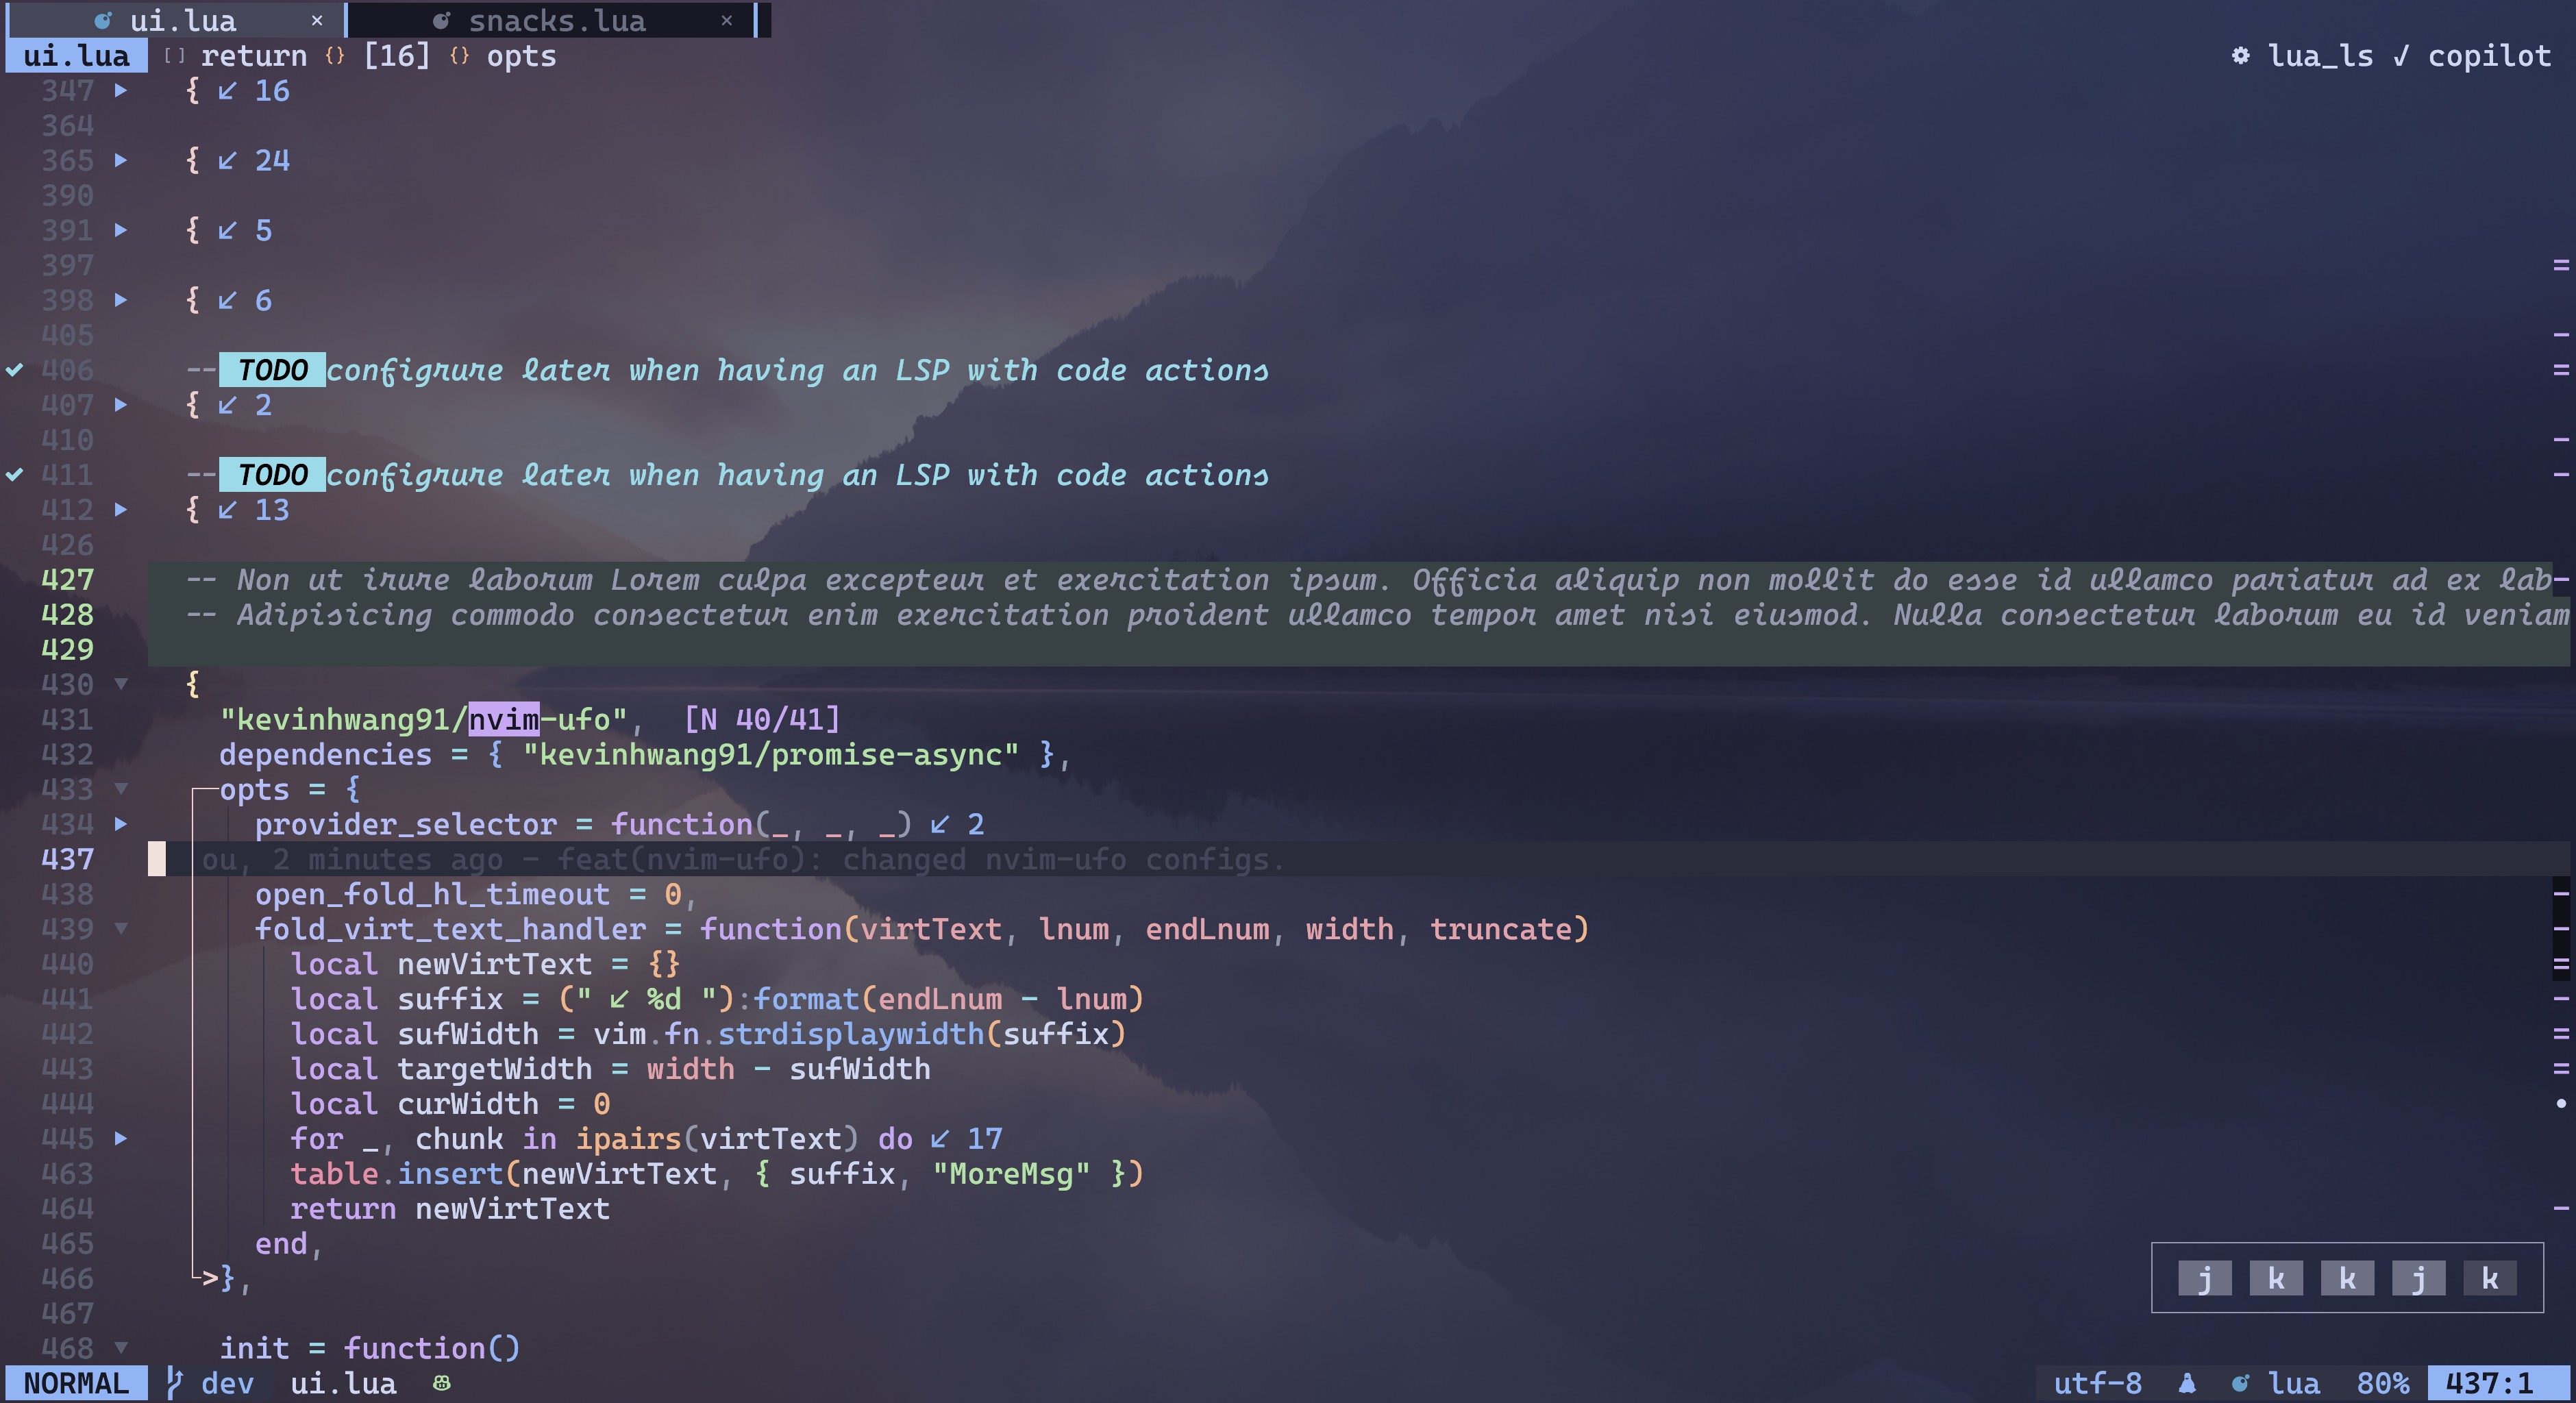
\includegraphics[width=0.75\linewidth]{./Figures/Final_Result.jpg}
  \end{figure}
\end{frame}

\begin{frame}
  \begin{itemize}
    \item 感谢:
      \begin{itemize}
        \item \link{Catppuccin}{https://catppuccin.com/} 
\includegraphics[height=10pt]{./Figures/Catppuccin_logo.png}
        \item \link{Catppuccin for beamer}{https://github.com/atticus-sullivan/beamercolortheme}
      \end{itemize}
      \vspace{0.5cm}
    \item 本教程的全部材料可以在我的Github上找到
      \begin{itemize}
        \item Slides: \url{https://github.com/Jacky-Lzx/nvim.tutorial.slides}
        \item Config: \url{https://github.com/Jacky-Lzx/nvim.tutorial.config}
      \end{itemize}
  \end{itemize}
\end{frame}

\end{document}
